\PassOptionsToPackage{table}{xcolor}
\documentclass{article} % For LaTeX2e
\usepackage{iclr2027_conference,times}

% Optional math commands from https://github.com/goodfeli/dlbook_notation.
\input{math_commands.tex}

\usepackage{hyperref}
\usepackage{url}

% packages
\usepackage{xcolor}
\usepackage{newfloat}
\usepackage{listings}
\usepackage{algorithm}
\usepackage{algorithmic}
\usepackage{adjustbox}
\usepackage{graphicx}
\usepackage{flafter}
\usepackage{pgfplots}
\pgfplotsset{compat=1.18}
\usepackage{booktabs}
\usepackage{amssymb}
\usepackage[capitalize,noabbrev]{cleveref}

\definecolor{tablehead}{RGB}{238,247,247}
\definecolor{blue1}{RGB}{235,245,255}
\definecolor{blue2}{RGB}{200,225,255}
\definecolor{blue3}{RGB}{150,200,255}
\definecolor{blue4}{RGB}{90,160,255}


\title{OSTRA: Learning Multi-Stage Robot Manipulation through Object-State Transition Supervision}

% Authors must not appear in the submitted version. They should be hidden
% as long as the \iclrfinalcopy macro remains commented out below.
% Non-anonymous submissions will be rejected without review.

\author{Antiquus S.~Hippocampus, Natalia Cerebro \& Amelie P. Amygdale \thanks{ Use footnote for providing further information
about author (webpage, alternative address)---\emph{not} for acknowledging
funding agencies.  Funding acknowledgements go at the end of the paper.} \\
Department of Computer Science\\
Cranberry-Lemon University\\
Pittsburgh, PA 15213, USA \\
\texttt{\{hippo,brain,jen\}@cs.cranberry-lemon.edu} \\
\And
Ji Q. Ren \& Yevgeny LeNet \\
Department of Computational Neuroscience \\
University of the Witwatersrand \\
Joburg, South Africa \\
\texttt{\{robot,net\}@wits.ac.za} \\
\AND
Coauthor \\
Affiliation \\
Address \\
\texttt{email}
}

% The \author macro works with any number of authors. There are two commands
% used to separate the names and addresses of multiple authors: \And and \AND.
%
% Using \And between authors leaves it to \LaTeX{} to determine where to break
% the lines. Using \AND forces a linebreak at that point. So, if \LaTeX{}
% puts 3 of 4 authors names on the first line, and the last on the second
% line, try using \AND instead of \And before the third author name.

\newcommand{\fix}{\marginpar{FIX}}
\newcommand{\new}{\marginpar{NEW}}

%\iclrfinalcopy % Uncomment for camera-ready version, but NOT for submission.
\begin{document}


\maketitle

\begin{abstract}
Sparse supervision is a key challenge in multi-stage manipulation, with the lack of supervision over the past-to-future evolution of objects required by the policy being particularly critical. To address this issue, we introduce the Object-State Transition Map (\textbf{OST-Map}), a unified object-centric representation that organizes task-relevant objects as identity-consistent graphs and represents historical and future object states in a shared structured space. Building on OST-Map, we propose \textbf{OSTRA}, a diffusion-based Object-State Transition Reasoning Architecture that hierarchically predicts future object states, target TCP poses, and continuous action trajectories. OSTRA combines Transition-Guided Attention, which prioritizes historical object-state transitions during future-state prediction, with Staged Denoising, which progressively translates predicted object changes into robot subgoals and executable actions. Experiments on three simulation benchmarks and seven diverse real-world tasks demonstrate consistent improvements over representative imitation learning baselines. Further ablations validate the contributions of OST-Map and the proposed architectural designs.
\end{abstract}

\section{Introduction}
\label{sec:introduction}

% challenge in multi-stage manipulation √
Sparse supervision is a key challenge in imitation learning, particularly for multi-stage robot manipulation tasks~\citep{Zare2024Survey,Mandlekar2020Learning,Chen2023Sequential,Jain2025LongerHorizon}. Completing such tasks requires a policy not only to understand the environment at the current time step, but also to retain knowledge of the past---for example, whether prior subtasks succeeded and how key objects changed (Figure~\ref{fig:teaser}, left)~\citep{Kang2025Incorporating,Mark2026BPP}. Because an environment consists of objects, the policy must understand how these objects have changed over time. Therefore, the currently observed environment alone is insufficient for the policy to predict the most appropriate action. The policy must also be aware of object changes within the environment. We refer to this challenge as the object-state transition supervision gap.
% Sparse supervision 在 imitation learning 中是一个 key challenge，特别是在 multi-stage robot manipulation 这一特定的 robot manipulation 任务类型中。
% multi-stage robot manipulation 在完成任务时，不仅仅需要 policy 理解当前时刻的 environment，还需要 policy 知晓过往的信息，比如上一个任务是否已经成功，之前执行任务时 environment 发生了哪些会影响当前任务执行的变化，而 environment 是由 object 组成的，也就是说 policy 需要知晓 object 在 environment 中一段时间下经历了哪些变化。
% 因此，仅仅只有当前观测到的 environment 不足以支撑 policy 预测最合理的动作，policy 还需要知晓 environment 中 object 的变化，我们称之为 object-state transition supervision gap

% how existing works solve this √
Early imitation learning methods improve short-term action prediction through action chunking or limited observation windows, but do not explicitly capture long-horizon task-relevant state transitions~\citep{Zhao2023Learning, chi2024diffusionpolicy}. Recent approaches incorporate past information through observation histories, latent memories, or task progress \citep{Liang2021Finite, shi2025memoryvla, Mark2026BPP}. Others use future observations, goal states, or latent plans as additional supervision \citep{lynch2020play, Mandlekar2020Learning, belkhale2023plato}. However, these methods represent temporal information at observation, latent, or task level, providing limited supervision on individual-object evolution during execution. Our method bridges this gap by unifying both temporal directions at the object level. Specifically, it represents past object-state transitions as structured historical context and predicts future object states as auxiliary supervision, enabling the policy to reason about how task-relevant objects have changed and how they should evolve next.

\begin{figure}[t]
    \centering
    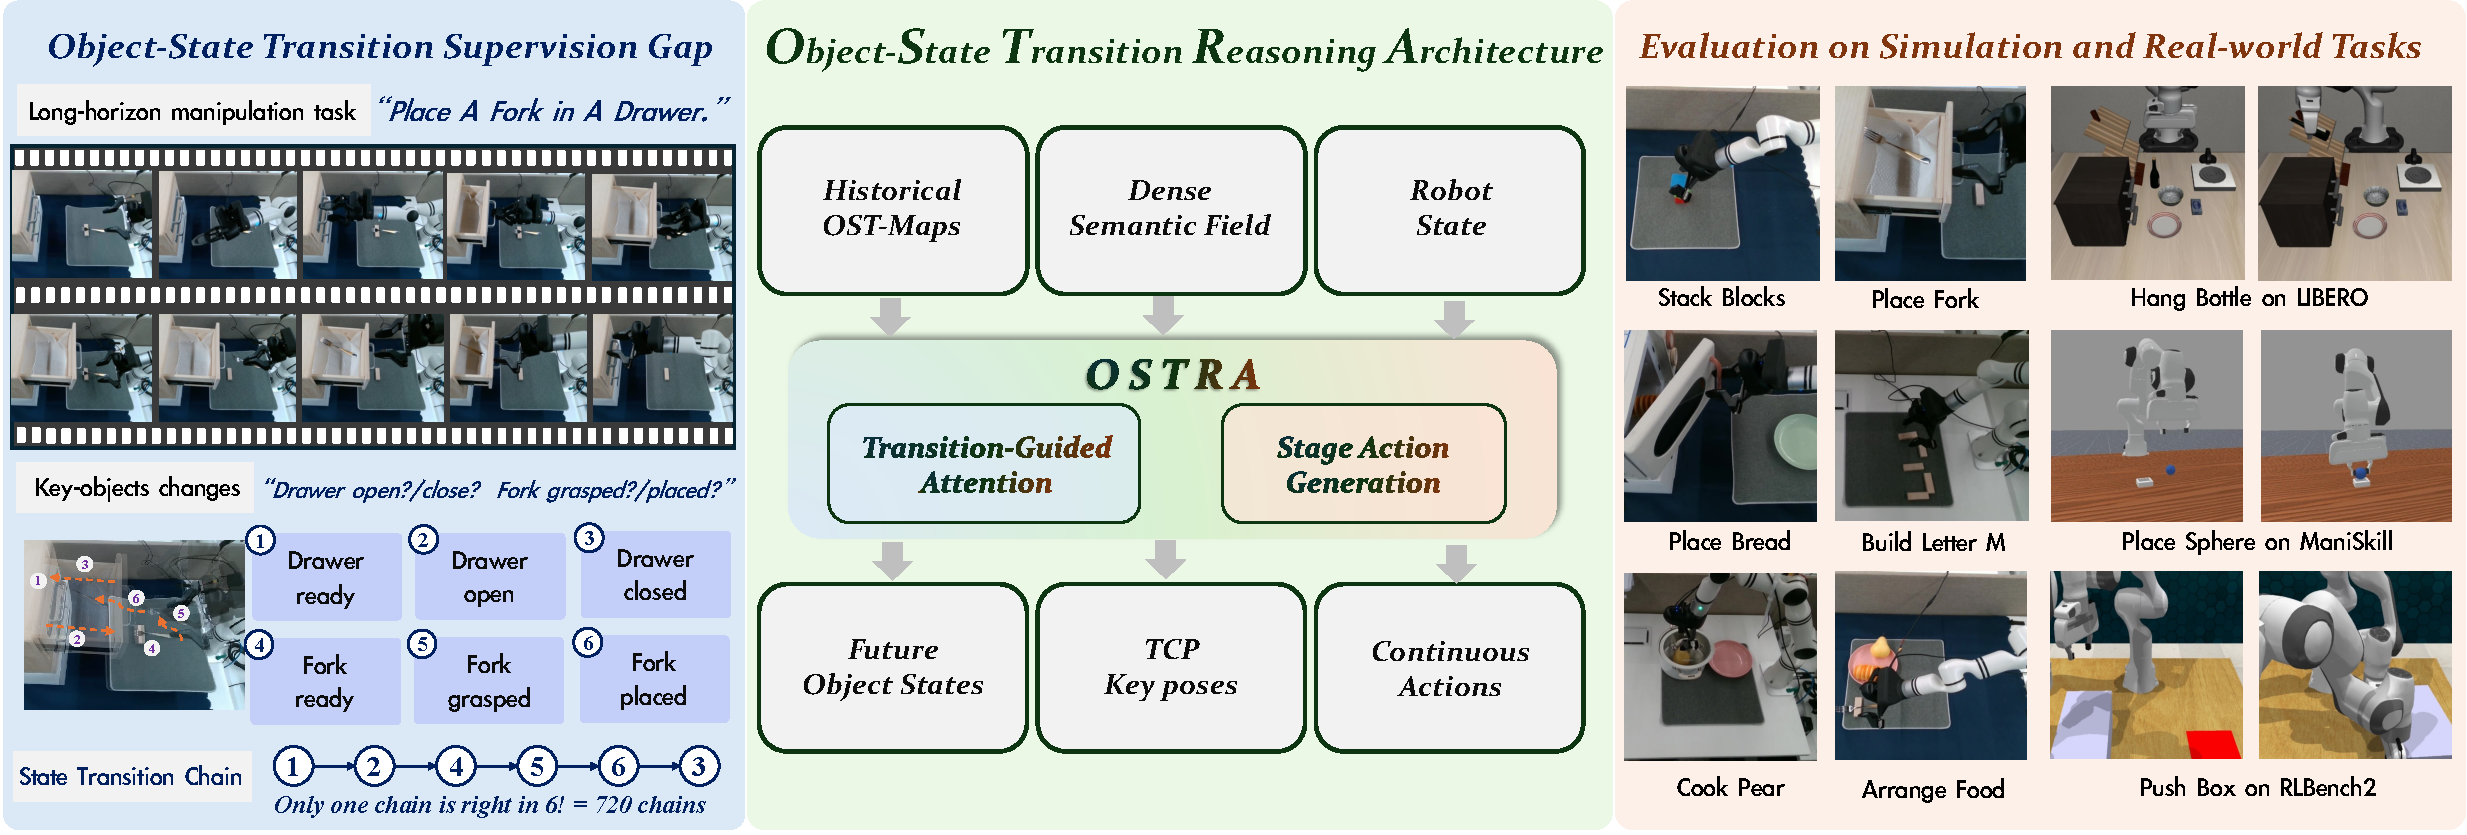
\includegraphics[width=\linewidth]{fig/1_teaser.pdf}
    \vspace{-20pt}
    \caption{\textbf{Overview of OSTRA.} Multi-stage manipulation requires
    resolving the object-state transition supervision gap: the policy must
    infer the correct transition chain from historical object changes. OSTRA
    combines historical OST-Maps, a dense Semantic Field, and the robot state
    to predict future object states, TCP keyposes, and continuous actions, and
    is evaluated across simulation and real-world tasks, where explicit
    transition supervision supports long-horizon control.}
    \vspace{-15pt}
    \label{fig:teaser}
\end{figure}



% OST-Map
To provide such supervision over past-to-future object evolution, we introduce the \textbf{O}bject-\textbf{S}tate \textbf{T}ransition Map (OST-Map), an object-centric representation of observed and future states in a shared structured space.
OST-Map avoids requiring policies to discover transition-relevant cues from visual histories using robot-centric action supervision alone.
Specifically, OST-Map represents each task-relevant object as an identity-consistent graph of structural nodes. Each node encodes its semantic identity, geometric parameters, and 6-DoF pose, while the graph edges capture structural and spatial relations among nodes and objects.
By preserving object and node identities across time, OST-Map organizes observations into temporally ordered object-centric tokens that explicitly characterize how task-relevant objects evolve. It further represents future object states in the same structured space, allowing the transition from historical to future object states to be directly supervised.
In this way, OST-Map turns otherwise implicit task progress and anticipated object changes into explicit intermediate targets between visual perception and robot action generation.

% OSTRA
Building on OST-Map, we introduce OSTRA, an \textbf{O}bject-\textbf{S}tate \textbf{T}ransition \textbf{R}easoning \textbf{A}rchitecture for multi-stage manipulation (Figure~\ref{fig:teaser}, middle).
OSTRA is a diffusion-based framework that hierarchically predicts future object states, target TCP poses, and continuous action trajectories.
It incorporates two key designs.
First, Transition-Guided Attention attends to historical OST-Map tokens before incorporating dense Semantic Field tokens, encouraging the model to prioritize task-relevant object-state transitions when predicting future states.
Second, Staged Denoising follows an object-to-TCP-to-action hierarchy that progressively translates predicted object-state changes into robot subgoals and executable actions.
Together, these designs connect object-level transition reasoning with robot-level planning and continuous control, enabling the policy to reason from how objects have changed to how they should evolve next and which actions should realize those changes.

We evaluate OSTRA on three simulation benchmarks and seven diverse real-world tasks.
Across these settings, OSTRA consistently improves over representative imitation learning baselines on multi-stage manipulation tasks.
Further ablation studies validate the contributions of OST-Map, Transition-Guided Attention, and Staged Denoising, demonstrating the effectiveness of structured object-state transition supervision for connecting scene evolution with robot action generation.

Our contributions are:
(1) To tackle the object-state transition supervision gap in multi-stage imitation learning, we introduce OST-Map, an object-centric representation that aligns historical object-state sequences with future object-state targets, enabling direct supervision of object-state transitions.
(2) Building on OST-Map, we introduce OSTRA, a diffusion-based architecture with two key designs.
    a) Transition-Guided Attention applies cross-attention to OST-Map tokens before Semantic Field tokens, encouraging the model to prioritize object-state transition information.
    b) Staged Denoising hierarchically predicts future object states, TCP poses, and action trajectories, progressively translating object-level state changes into robot subgoals and continuous control.
(3) We conduct evaluations across three simulation benchmarks and seven diverse real-world tasks, demonstrating consistent performance gains over representative imitation learning baselines.
% Further ablation studies validate the contributions of OST-Map, Transition-Guided Attention, and Staged Denoising, confirming the effectiveness of structured object-state transition supervision for multi-stage manipulation.

\section{Related Work}
\label{sec:related_work}

\subsection{Long-Horizon Visuomotor Imitation Learning}

Long-horizon manipulation requires coherent behavior over extended execution.
Existing methods shorten the control horizon through action chunking,
autoregressive prediction, or diffusion-based
action generation~\citep{Zhao2023Learning,chi2024diffusionpolicy,
Haldar2025BAKU,reuss2024multimodal}. Other approaches introduce higher-level
task structure through subgoals, skill composition, progress estimation, or
planning~\citep{shiarlis2018taco,gupta2019relay,Chen2023Sequential,
Kang2025Incorporating,Jain2025LongerHorizon,Liu2026PALM,
Zhang2026AtomicVLA,Feng2025ReflectivePlanning,Zhou2026Act2Goal}.
These methods organize actions or task stages over time, but generally do not
supervise how task-relevant objects evolve from historical to target states.

\subsection{Temporal Modeling in Robot Policies}

Temporal context is commonly incorporated through observation histories,
latent memories, recurrent features, or retrieved past
frames~\citep{Liang2021Finite,Fang2025SAM2Act,shi2025memoryvla,
Mark2026BPP}. Recent policies further maintain recurrent or hierarchical
memory to capture dependencies beyond the current
observation~\citep{Ji2026HiMe,Xiao2026AVAVLA,Li2026OptimusVLA}.

A complementary direction uses future information as guidance.
Existing methods condition policies on goal observations or latent plans
~\citep{lynch2020play,Mandlekar2020Learning}, predict future visual states or
joint video-action trajectories~\citep{Hu2025VPP,Zhu2025UWM}, or learn
predictive representations from future transitions and interaction targets
~\citep{Zeng2024MPI}. Despite using historical and future context, these
approaches represent time through holistic observations, latent memories,
predicted frames, or task-level targets rather than identity-consistent state
transitions of individual objects.

\subsection{Object-Centric Representations for Manipulation}

Object-centric policies organize perception and action around manipulable
entities. Existing approaches use object
proposals or 3D object features as policy inputs
~\citep{zhu2022viola,zhu2023learning}, learn affordance-, flow-, or
contact-based interaction representations
~\citep{belkhale2023plato,xu2024im2flow2act,Zhang2026AffordGen,
Lee2025ViTaSCOPE}, or represent manipulation through explicit object motion,
including SE(3) pose trajectories and object pointflow
~\citep{Hsu2025SPOT,Yang2025PPI}. Recent work also introduces structured
object-level representations based on physical concepts or
semantic operations~\citep{Wei2026PhysicalConcepts,Tang2026SEAM}.

Object-centric world models use entity-level representations for dynamics and
future prediction
~\citep{ferraro2025focus,jeong2025ocwm}, while graph-based
approaches preserve explicit objects and relations for manipulation planning
~\citep{zhu2026orion}. These methods typically represent objects as perceptual
units, interaction interfaces, motion variables, or future prediction targets.
In contrast, OST-Map maintains identity-consistent structural states across
observed and future task stages, making past-to-future object-state transitions
explicit supervision for action generation.

\section{Method}
\label{sec:method}

\begin{figure}[t]

    \centering
    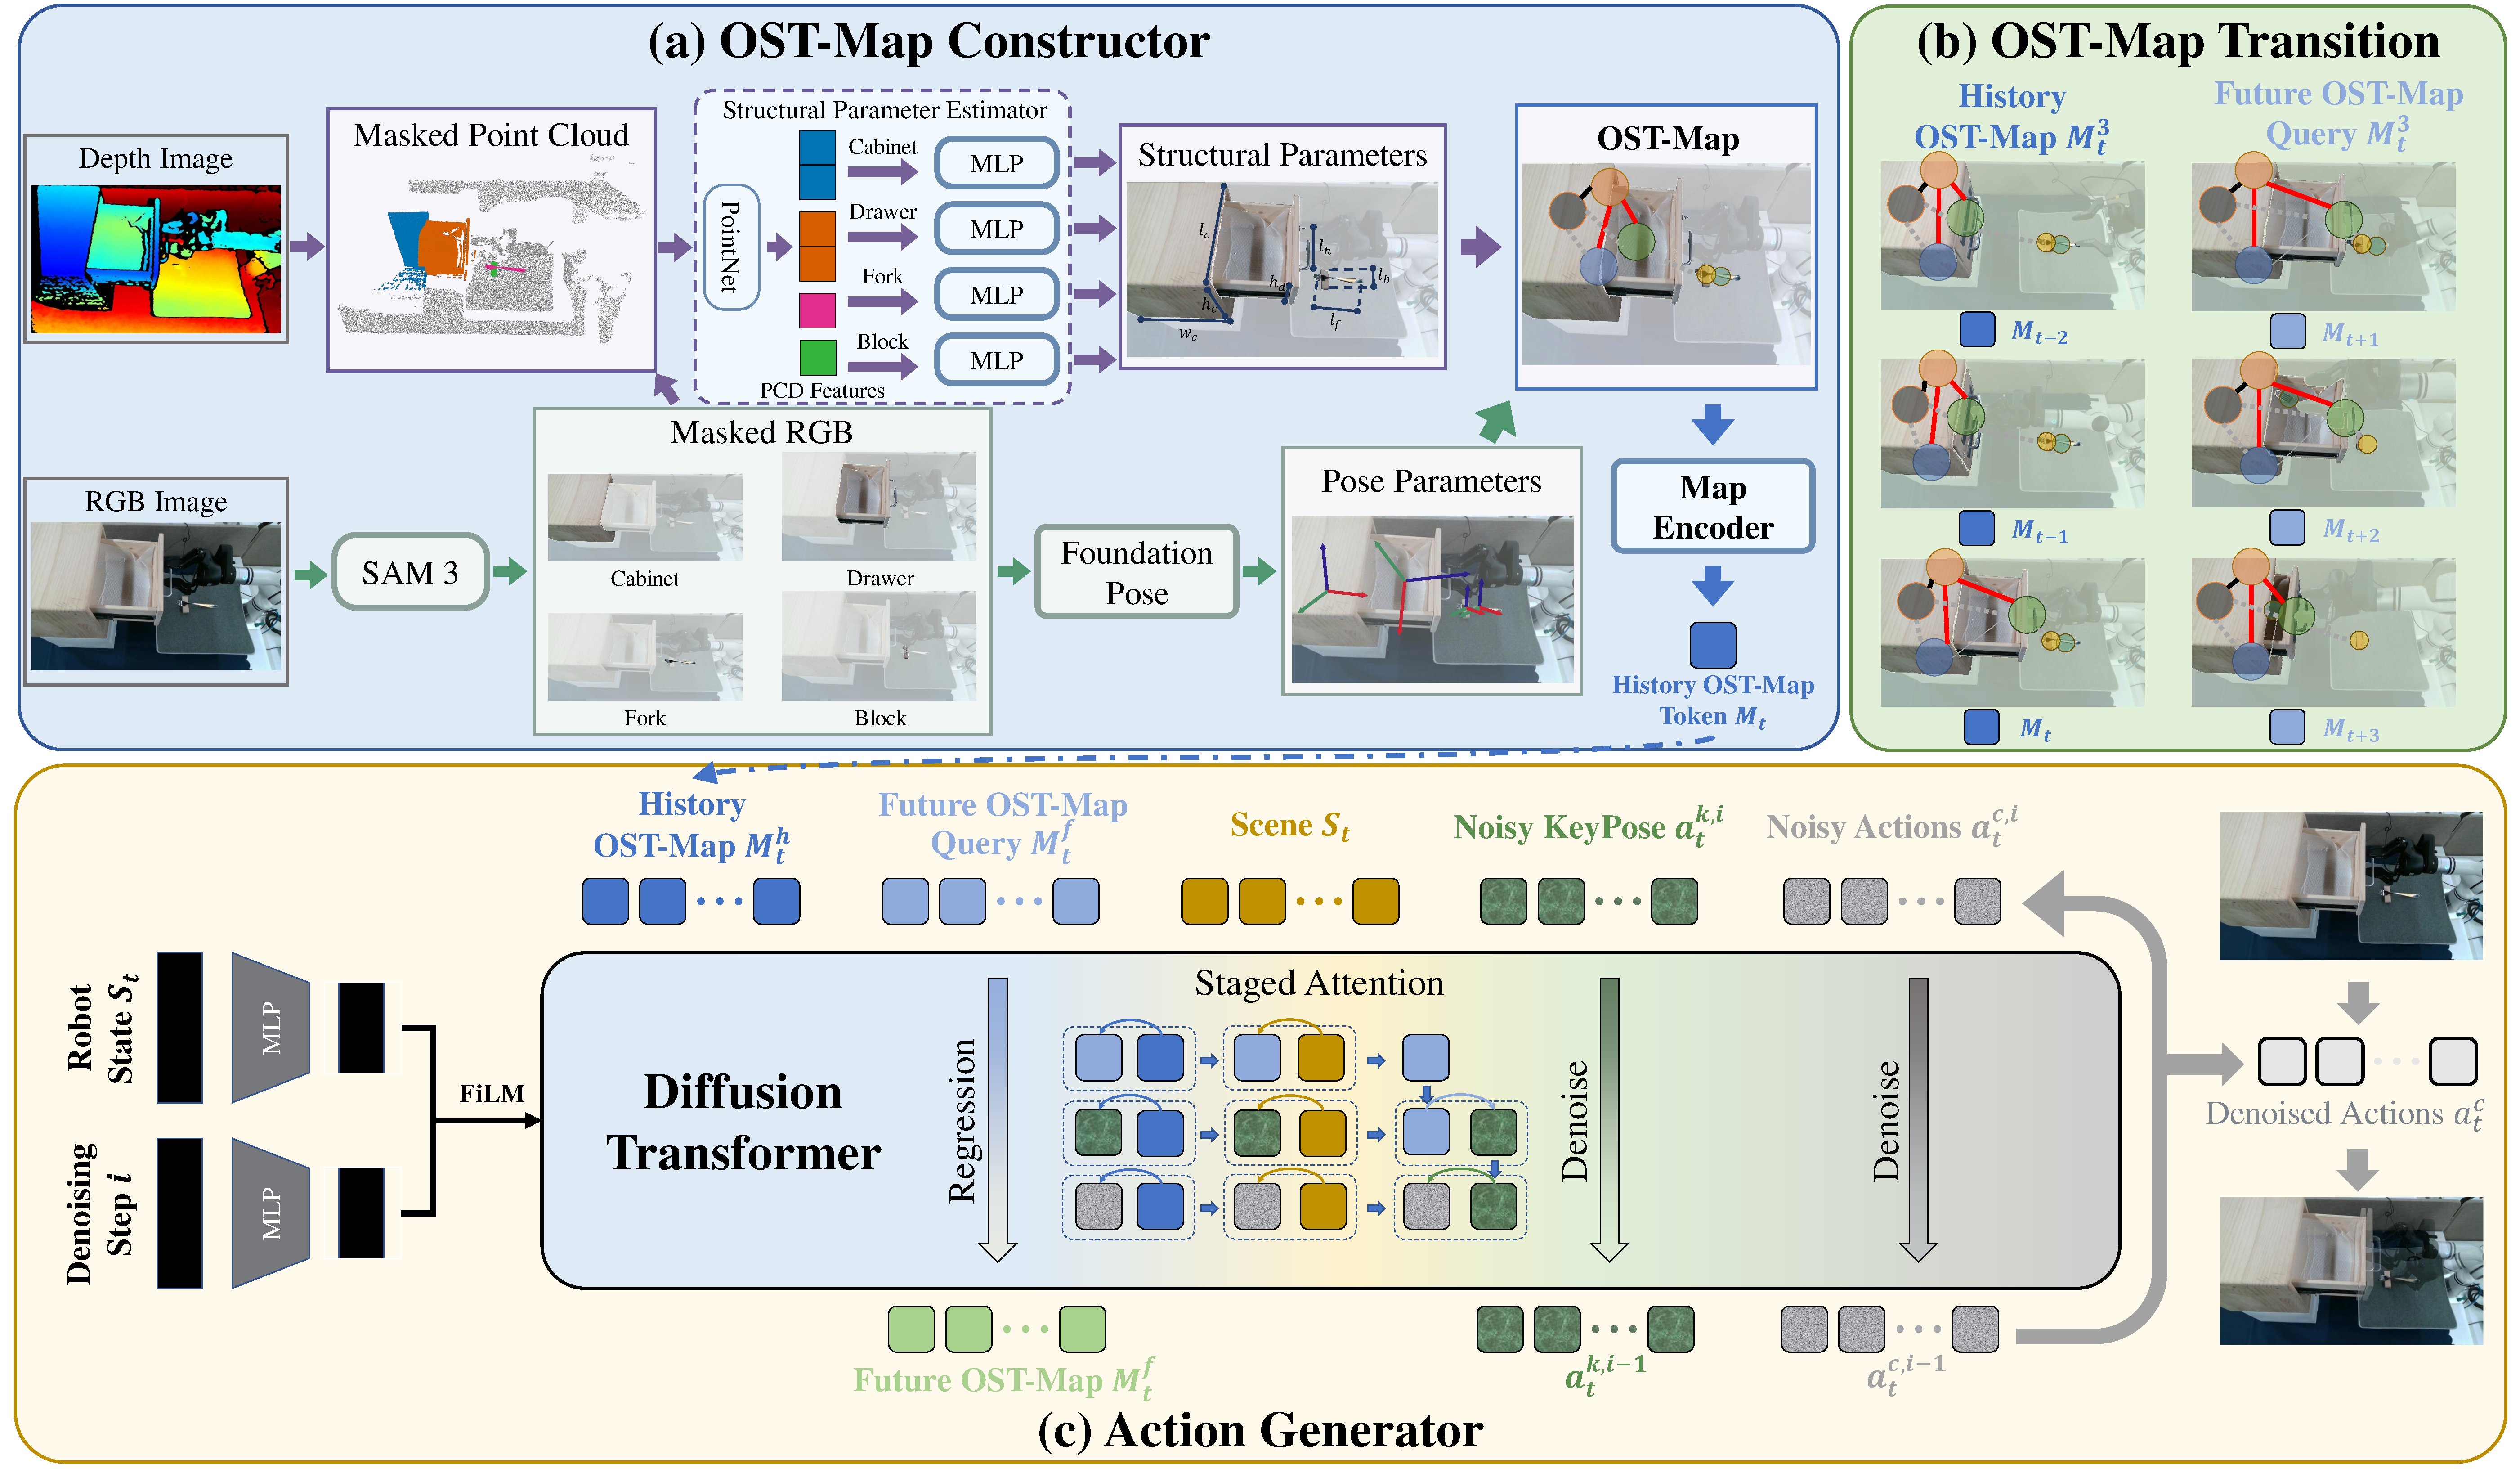
\includegraphics[width=\textwidth]{fig/2_pipeline.pdf}
    \vspace{-20pt}
    \caption{
    \textbf{Overview of OSTRA.}
    \textbf{(a) OST-Map Constructor:} RGB-D observations are converted into
    identity-consistent object-centric maps by estimating task-relevant object masks,
    structural parameters, and 6-DoF poses.
    \textbf{(b) Object-State Transition Modeling:} temporally aligned historical
    OST-Maps provide explicit object-state transition context and are used to query
    future object states.
    \textbf{(c) Transition-Guided Action Generation:} historical OST-Map tokens,
    future object-state queries, dense Semantic Field tokens, robot states, and the
    diffusion timestep are processed by OSTRA, which progressively predicts future
    object states, TCP keyposes, and continuous actions following the hierarchy
    \emph{object state $\rightarrow$ TCP subgoal $\rightarrow$ action} for
    structured multi-stage control.
    }
    \label{fig:ostra_pipeline}
    \vspace{-12pt}
\end{figure}


\subsection{Overview}
\label{sec:method_overview}

\textbf{Problem Formulation.}
We consider multi-stage robot manipulation from RGB-D observations.
At time $t$, the policy receives an observation window
$\mathcal{O}_{t}=\{(I_{\tau},D_{\tau},s_{\tau})\}_{\tau=t-T_o+1}^{t}$
and predicts an action chunk
$A_t=\{a_{t+k}\}_{k=0}^{H_a-1}$.
Rather than directly mapping the current visual observation to robot actions,
OSTRA explicitly models how task-relevant objects have evolved throughout the
observation history and which object states should be achieved next.

\textbf{Object-State Transition Modeling.}
As shown in \cref{fig:ostra_pipeline}, each RGB-D observation is converted into
an OST-Map whose identity-consistent nodes encode object semantics, structure,
affordance, and 6-DoF pose. Tracking yields aligned historical maps that expose
object-state transitions and supervise future states in the same structured
space, while a dense Semantic Field preserves local scene evidence.

\textbf{Transition-Guided Action Generation.}
Transition-Guided Attention first grounds prediction queries in historical
OST-Map tokens and then incorporates dense Semantic Field tokens. Staged Action
Generation follows the hierarchy
\emph{object state $\rightarrow$ TCP subgoal $\rightarrow$ action}:
future OST-Map keyframes condition TCP-keyframe denoising, whose representation
then conditions continuous-action generation.


\subsection{OST-Map: Object-State Transition Map}
\label{sec:ost_map}

\begin{figure}[t]
    \centering
    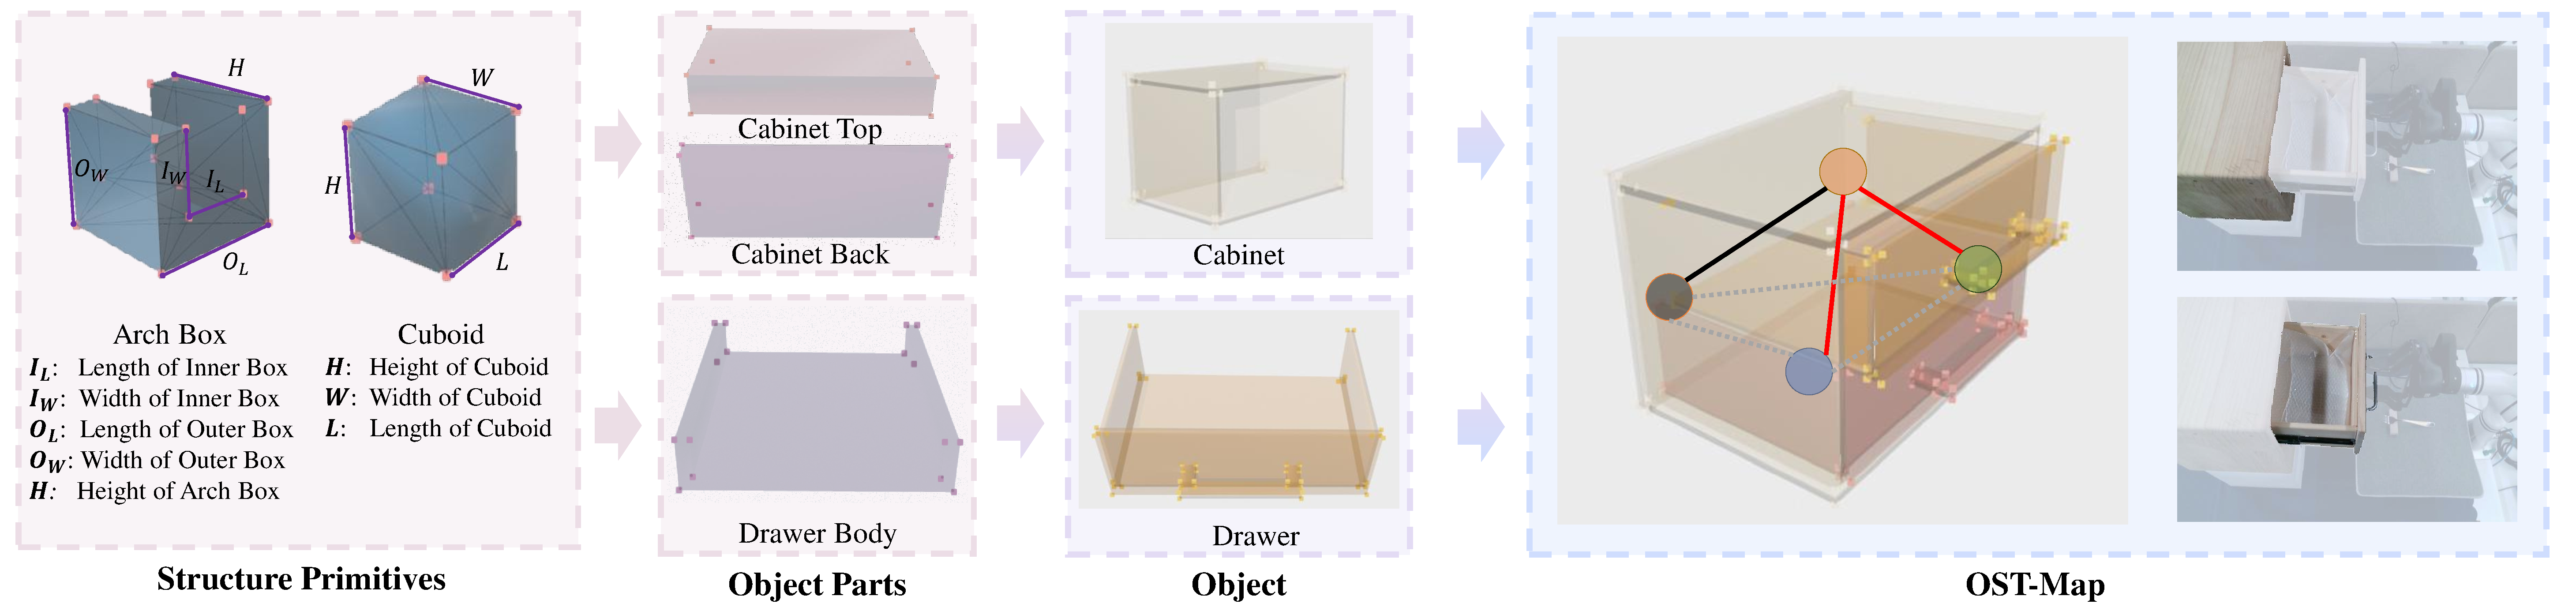
\includegraphics[width=\textwidth]{fig/3_ostmap.pdf}
    \vspace{-20pt}
    \caption{
    \textbf{Representation of OST-Map.}
    Parameterized structure primitives are composed into object parts and
    further assembled into task-relevant objects.
    Each object is represented by identity-consistent structural nodes and
    their relations, while node poses evolve with manipulation.
    The resulting OST-Map provides a compact object-centric representation of
    scene structure and object-state transitions for temporally grounded,
    multi-stage action generation.
    }
    \label{fig:ost_map}
    \vspace{-12pt}
\end{figure}

As illustrated in \cref{fig:ost_map}, OST-Map composes parameterized primitives
into object parts and identity-consistent structural nodes. Persistent node
identities preserve fine-grained structure and enable temporal tracking.

For a task with $N$ structural nodes, the OST-Map at time $t$ is defined as
an attributed graph
$\mathcal{M}_t=(\mathcal{V}_t,\mathcal{E}_t)$.
Each node $v_{t,i}\in\mathcal{V}_t$ is represented as
\begin{equation}
    v_{t,i}
    =
    \bigl(
    c_i,\mathcal{P}_i,\mathcal{A}_i,p_{t,i},q_{t,i}
    \bigr),
    \label{eq:ost_node}
\end{equation}
where $c_i$ denotes its semantic identity,
$\mathcal{P}_i$ and $\mathcal{A}_i$ denote its structural and affordance point
sets, and
$(p_{t,i},q_{t,i})\in\mathbb{R}^{3}\times\mathbb{S}^{3}$
denotes its 6-DoF pose.
Semantic identity and local structural attributes remain fixed within an
episode, while pose evolves with the object state.

Each edge $e_{t,ij}\in\mathcal{E}_t$ stores its relation type, parameters,
reference anchors, and relative pose. Free-relation edges connect pairs without
task-specific relations. The sequence $\mathcal{M}_{t-T_o+1:t}$ captures
object-state evolution in an identity-aligned space.


\subsection{OSTRA: Object-State Transition Reasoning Architecture}
\label{sec:ostra}

\textbf{OST-Map Construction and Transition Targets.}
As shown in \cref{fig:ostra_pipeline}(a), OSTRA first constructs an OST-Map
from each RGB-D observation. SAM 3~\citep{sam3} segments prompted task objects,
FoundationPose~\citep{foundationposewen2024} registers and tracks their 6-DoF
poses, and PointNet~\citep{Qi2017PointNet} with object-specific MLP heads
estimates structural parameters from masked point clouds, producing a
temporally aligned map sequence.

Historical OST-Maps encode observed transitions. During training, the
structural-node positions at the next $H_k$ task keyframes define future-state
targets, 
\begin{equation}
    Y_t^{M}
    =
    \{p^{\star}_{t,h,i}\}_{h=1,i=1}^{H_k,N}.
    \label{eq:future_map_target}
\end{equation}
paired with TCP keyframes $Y_t^{E}$ and action chunk $A_t$. Future observations
provide training-only supervision, while the shared OST-Map space supplies
identity-aligned transition targets.


\textbf{Multimodal Context Encoding.}
OSTRA combines a sparse OST-Map with a dense Semantic Field. Depth points
$X_t=\{x_{t,j}\}_{j=1}^{P}$ are paired with image-aligned pretrained DINO
features $d_{t,j}$. PointNet++ encodes
$\operatorname{concat}(x_{t,j},d_{t,j})$ into dense tokens
$F_t^{S}$ for cross-attention and downsampled tokens $\bar{F}_t^{S}$ for compact
planning context.

For each historical map, node embeddings combine PointNet features of
$\mathcal{P}_i$ and $\mathcal{A}_i$ with semantic, pose, temporal, and identity
embeddings. Edge embeddings encode relation attributes and relative pose. A
graph transformer produces coordinate-aware map tokens $F_t^{M}$. Map and scene
tokens retain 3D coordinates for relative spatial attention. Robot state and
diffusion timestep condition prediction blocks through adaptive normalization.


\textbf{Transition-Guided Attention.}
A central challenge is the large imbalance between the sparse OST-Map tokens
and the dense Semantic Field tokens.
Directly mixing them in a single attention context can weaken the structured
transition cues carried by the OST-Map.
OSTRA therefore introduces \emph{Transition-Guided Attention}, in which each
prediction query first attends to historical OST-Map tokens and subsequently
to the dense Semantic Field:
\begin{equation}
    \widetilde{Z}
    =
    \operatorname{CA}(Z,F^{M}),
    \qquad
    Z^{+}
    =
    \operatorname{CA}(\widetilde{Z},F^{S}),
    \label{eq:tga}
\end{equation}
where $\operatorname{CA}$ denotes cross-attention.
Cross-attention uses relative 3D rotary encodings computed from query and
context coordinates.

For future object-state prediction, queries repeat the latest structural-node
coordinates over the next $H_k$ keyframes
and augmenting them with learned keyframe-time and node-identity embeddings.
TCP and action queries come from their noisy diffusion variables. The map-first
order preserves transition grounding before introducing denser visual context.

\begin{table}[t]
    \vspace{-10pt}
    \centering
    \caption{\textbf{Summary of the main simulation results.}
    We report average task success rate (\%) on each benchmark.
    Full per-task results are in Appendix~\ref{app:full_sim_results}.
    \textbf{Bold} and \underline{underlining} denote the best and second-best
    results, respectively, under the benchmark-specific evaluation protocols.}
    \label{tab:main_results_summary}
    \vspace{2pt}
    \small
    \setlength{\tabcolsep}{6pt}
    \begin{adjustbox}{max width=\textwidth}
    \begin{tabular}{lc|lc|lc}
        \toprule
        \rowcolor{tablehead}
        \multicolumn{2}{c|}{RLBench2~\citep{James2020RLBench} (7 tasks)} &
        \multicolumn{2}{c|}{ManiSkill~\citep{Gu2023ManiSkill2} (6 tasks)} &
        \multicolumn{2}{c}{LIBERO~\citep{liu2023libero} (40 tasks)} \\
        \rowcolor{tablehead}
        Method & Mean S.R. (\%) & Method & Mean S.R. (\%) & Method & Mean S.R. (\%) \\
        \midrule
        ACT~\citep{Zhao2023Learning} & 15.5 &
        ACT~\citep{Zhao2023Learning} & 21.3 &
        ACT~\citep{Zhao2023Learning} & 67.7 \\
        DP3~\citep{Ze2024DP3} & 26.0 &
        Diffusion Policy~\citep{chi2024diffusionpolicy} & 26.8 &
        GROOT~\citep{zhu2023learning} & 66.2 \\
        3D Diffuser Actor~\citep{ke2024diffuseractor} & 64.7 &
        DP3~\citep{Ze2024DP3} & 53.8 &
        Diffusion Policy~\citep{chi2024diffusionpolicy} & 72.4 \\
        PerAct$^2$~\citep{shridhar2022peract} & 40.0 &
        3D Diffuser Actor~\citep{ke2024diffuseractor} & 51.5 &
        BAKU~\citep{Haldar2025BAKU} & 93.0 \\
        PPI~\citep{Yang2025PPI} & 80.8 &
        \underline{PPI~\citep{Yang2025PPI}} & \underline{56.8} &
        MDT~\citep{reuss2024multimodal} & 76.1 \\
        Diffusion Policy~\citep{chi2024diffusionpolicy} & 42.6 &
        BAKU~\citep{Haldar2025BAKU} & 43.0 &
        DP3~\citep{Ze2024DP3} & 73.0 \\
        \underline{SAM2Act+~\citep{Fang2025SAM2Act}} & \underline{84.5} &
        FlowPolicy~\citep{zhang2024flowpolicy} & 39.5 &
        UWM~\citep{Zhu2025UWM} & 91.8 \\
        GROOT~\citep{zhu2023learning} & 45.2 &
        SPOT~\citep{Hsu2025SPOT} & 47.5 &
        \underline{MemoryVLA~\citep{shi2025memoryvla}} & \underline{96.7} \\
        SPOT~\citep{Hsu2025SPOT} & 82.3 &
        Im2Flow2Act~\citep{xu2024im2flow2act} & 45.7 &
        BPP~\citep{Mark2026BPP} & 90.9 \\
        \rowcolor{tablehead}
        \textbf{OSTRA (Ours)} & \textbf{89.8} &
        \textbf{OSTRA (Ours)} & \textbf{74.5} &
        \textbf{OSTRA (Ours)} & \textbf{97.4} \\
        \bottomrule
    \end{tabular}
    \end{adjustbox}
    \vspace{-8pt}
\end{table}


\begin{algorithm}[h]
\caption{Staged Action Generation in OSTRA}
\label{alg:ostra_generation}
\begin{algorithmic}[1]
\REQUIRE Map context $F^M$, scene context $F^S$, robot state $s_t$
\ENSURE Action chunk $\widehat{A}_t$

\STATE Construct future object queries $Z^M$
\STATE Initialize $Y^{E,N},A^N\sim\mathcal{N}(0,I)$

\FOR{$n=N,\ldots,1$}
    \STATE $P^M,\widehat{Y}^M_n
    \leftarrow \textsc{ObjectStage}(Z^M,F^M,F^S,s_t,n)$

    \STATE $P^E,\widehat{\epsilon}^E_n
    \leftarrow \textsc{TCPStage}(Y^{E,n},F^M,F^S,\operatorname{sg}(P^M),s_t,n)$

    \STATE $P^A,\widehat{\epsilon}^A_n,\widehat{G}_n
    \leftarrow \textsc{ActionGenerator}(A^n,F^M,F^S,\operatorname{sg}(P^E),s_t,n)$

    \STATE $Y^{E,n-1}
    \leftarrow \textsc{Denoise}(Y^{E,n},\widehat{\epsilon}^E_n,n)$

    \STATE $A^{n-1}
    \leftarrow \textsc{Denoise}(A^n,\widehat{\epsilon}^A_n,n)$
\ENDFOR

\RETURN $A^0$ with predicted gripper states
\end{algorithmic}
\end{algorithm}
\vspace{-8pt}

\textbf{Staged Action Generation.}
As illustrated in \cref{fig:ostra_pipeline}(c), OSTRA translates
object-state transitions into executable robot motion through the hierarchy
\emph{object state $\rightarrow$ TCP subgoal $\rightarrow$ action}.
At each diffusion step, future-object queries yield an object plan $P^{M}$ and
predicted states $\widehat{Y}^{M}$. Noisy TCP queries then combine ordered
map-to-scene attention with $\operatorname{sg}(P^{M})$ to produce a TCP plan
$P^{E}$ and TCP-noise estimate. Finally, the Action Generator conditions noisy
action queries on $\operatorname{sg}(P^{E})$ to predict action noise and
gripper openness. TCP
keyframes and actions are progressively denoised from Gaussian noise, whereas
future object states are re-predicted at every step. Position and rotation use
separate schedules. Algorithm~\ref{alg:ostra_generation} summarizes the procedure.


\textbf{Training Objective and Inference.}
OSTRA is trained with direct supervision at all three levels of the hierarchy.
The objective combines future object-state prediction, TCP diffusion, action
diffusion, and gripper supervision:
\begin{equation}
\begin{split}
    \mathcal{L} ={}&
    \lambda_M
    \lVert\widehat{Y}^{M}-Y^{M}\rVert_1
    +
    \lambda_E
    \lVert\widehat{\epsilon}_{E}-\epsilon_E\rVert_1 \\
    &+
    \lambda_A
    \lVert\widehat{\epsilon}_{A}-\epsilon_A\rVert_1
    +
    \lambda_G
    \lVert\widehat{G}-G\rVert_1 .
\end{split}
\label{eq:total_loss}
\end{equation}
The terms supervise object evolution, TCP subgoals, continuous control, and
gripper state. Stop-gradient requires each stage to satisfy its own target.

At inference, map and field contexts are encoded once per replanning step. Each
reverse step executes Algorithm~\ref{alg:ostra_generation}. The policy
executes the first predicted actions and replans from the updated history.

\section{Experiments}
\label{sec:experiments}

Our experiments address five questions:
\textbf{Q1:} Does OSTRA outperform baseline policies across simulation
benchmarks (\cref{sec:simulation_experiments})?
\textbf{Q2:} Do these benefits hold in real-world manipulation
(\cref{sec:real_world_experiments})?
\textbf{Q3:} How do errors and computational costs in the foundation-model
components affect OSTRA? We study their impact on task success in
\cref{sec:system_error_breakdown} and their latency in \cref{sec:latency}.
\textbf{Q4:} Which architectural designs contribute to performance?
\textbf{Q5:} How sensitive is OSTRA to its key hyperparameters?
The last two questions are addressed by the design ablations and
hyperparameter analysis in \cref{sec:ablation_studies}.

\begin{figure}[t]
    \centering
    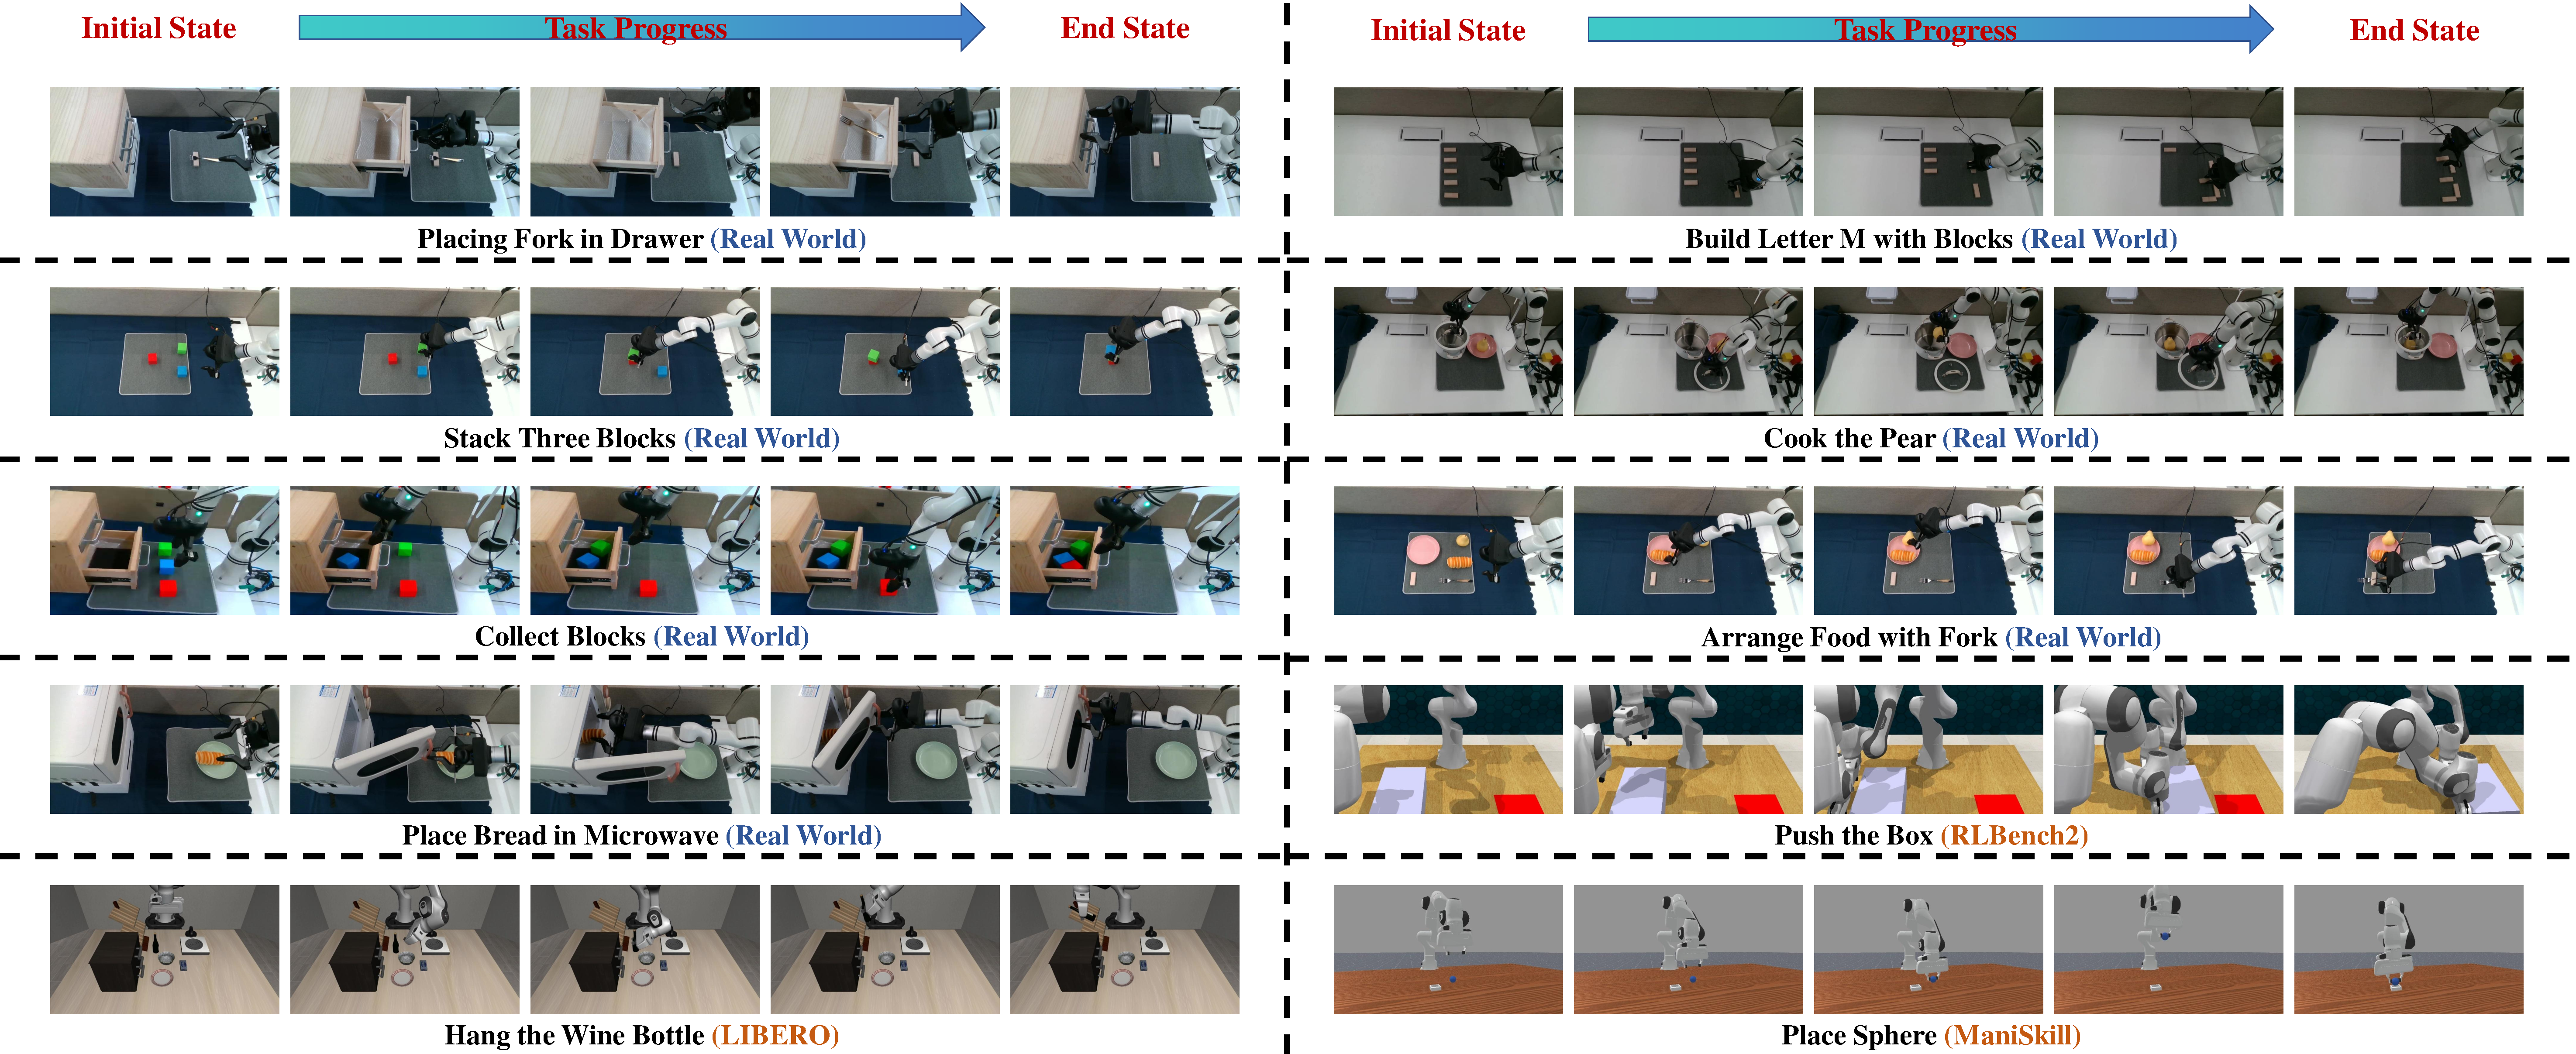
\includegraphics[width=\textwidth]{fig/4_demonstration.pdf}
    \vspace{-20pt}
    \caption{Task demonstrations from initial state to task completion.
    The seven real-world tasks are \textit{Place Fork in Drawer},
    \textit{Stack Three Blocks}, \textit{Collect Blocks},
    \textit{Place Bread in Microwave}, \textit{Build Letter M with Blocks},
    \textit{Cook the Pear}, and \textit{Arrange Food with Fork}.
    The figure also shows representative tasks from the three simulation
    benchmarks: \textit{Push the Box} from
    RLBench2~\citep{James2020RLBench}, \textit{Place Sphere} from
    ManiSkill~\citep{Gu2023ManiSkill2}, and \textit{Hang the Wine Bottle}
    from LIBERO~\citep{liu2023libero}, together spanning articulated,
    contact-rich, and long-horizon robot manipulation challenges.}
    \label{fig:demonstration}
    \vspace{-12pt}
\end{figure}

\begin{table*}[t]
    % \vspace{-6pt}
    \centering
    \caption{\textbf{Real-world manipulation results.}
    We report full-task success rate (\%) over 20 trials per task and the
    average across seven tasks. \textbf{Bold} and \underline{underlining}
    denote the best and second-best results, respectively, using identical
    trial counts for every policy in the matched comparison.}
    \label{tab:real_world_results}
    \vspace{2pt}
    \scriptsize
    \setlength{\tabcolsep}{4pt}
    \resizebox{\textwidth}{!}{%
    \begin{tabular}{lcccccccc}
        \toprule
        \rowcolor{tablehead}
        Method
        & Avg. $\uparrow$
        & \shortstack{Place Fork\\in Drawer}
        & \shortstack{Stack Three\\Blocks}
        & \shortstack{Arrange Food\\with Fork}
        & \shortstack{Place Bread\\in Microwave}
        & \shortstack{Build Letter M\\with Blocks}
        & \shortstack{Collect\\Blocks}
        & \shortstack{Cook the\\Pear} \\
        \midrule
        ACT~\citep{Zhao2023Learning}                    & 19.3 & 15 & 10 & 35 & 20 &  0 & 30 & 25 \\
        Diffusion Policy~\citep{chi2024diffusionpolicy} & 20.0 & 10 &  5 & 40 & 20 &  0 & 35 & 30 \\
        DP3~\citep{Ze2024DP3}                           & 40.7 & 40 & 20 & 65 & 45 &  0 & 60 & 55 \\
        PPI~\citep{Yang2025PPI}                         & 50.7 & 50 & 30 & 75 & 55 & 10 & 70 & 65 \\
        SAM2Act+~\citep{Fang2025SAM2Act}                & \underline{59.3} & \underline{55} & \underline{40} & \underline{85} & \underline{65} & \underline{15} & \underline{80} & \underline{75} \\
        MemoryVLA~\citep{shi2025memoryvla}              & 54.3 & 50 & 35 & 80 & 60 & 10 & 75 & 70 \\
        MPI~\citep{Zeng2024MPI}                         & 44.3 & 45 & 25 & 70 & 50 &  0 & 65 & 55 \\
        SPOT~\citep{Hsu2025SPOT}                        & 52.1 & 45 & 35 & 80 & 55 & 10 & 75 & 65 \\
        Im2Flow2Act~\citep{xu2024im2flow2act}           & 42.9 & 40 & 25 & 70 & 45 &  5 & 60 & 55 \\
        \midrule
        \rowcolor{tablehead} 
        OSTRA (Ours)                                    & \textbf{84.3} & \textbf{85} & \textbf{80} & \textbf{95} & \textbf{85} & \textbf{65} & \textbf{90} & \textbf{90} \\
        \bottomrule
    \end{tabular}%
    }
    \vspace{-6pt}
\end{table*}


\begin{table}[t]
\vspace{-6pt}
\centering
\caption{System error breakdown for OSTRA. We use ground-truth replacements to
identify the dominant bottleneck in OST-Map construction. Ground-truth quantities
are used only for analysis and are not part of the inference interface.
$\Delta$ reports the improvement over Full OSTRA.}
\label{tab:system_breakdown}
\vspace{2pt}
\small
\setlength{\tabcolsep}{6pt}
\begin{adjustbox}{max width=0.9\columnwidth}
\begin{tabular}{l|ccc|>{\columncolor{white}}c|c}
\toprule
Setting & GT Extraction & GT Object Pose & GT Structural Size & Avg. Success & $\Delta$ \\
\midrule
Full OSTRA & & & & \cellcolor{blue1}89.8 & 0.0 \\
+ GT Extraction & $\checkmark$ & & & \cellcolor{blue1}90.3 & +0.5 \\
+ GT Object Pose & & $\checkmark$ & & \cellcolor{blue2}91.9 & +2.1 \\
+ GT Structural Size & & & $\checkmark$ & \cellcolor{blue2}93.4 & +3.6 \\
+ GT Extraction + GT Object Pose & $\checkmark$ & $\checkmark$ & &
\cellcolor{blue2}92.1 & +2.3 \\
+ GT Extraction + GT Structural Size & $\checkmark$ & & $\checkmark$ &
\cellcolor{blue3}94.2 & +4.4 \\
+ GT Object Pose + GT Structural Size & & $\checkmark$ & $\checkmark$ &
\cellcolor{blue4}95.7 & +5.9 \\
+ GT Extraction + GT Object Pose + GT Structural Size
& $\checkmark$ & $\checkmark$ & $\checkmark$
& \cellcolor{blue4}96.4 & +6.6 \\
\bottomrule
\end{tabular}
\end{adjustbox}
\vspace{-8pt}
\end{table}


\begin{table}[t]
    % \vspace{-6pt}
    \centering
    \caption{\textbf{Inference latency (ms) and throughput.}
    We report mean component and end-to-end latency for the first frame and
    subsequent frames at batch size one. The first frame initializes OST-Map.
    Subsequent frames track objects and update the map for end-to-end comparison.}
    \label{tab:latency}
    \vspace{2pt}
    \footnotesize
    \renewcommand{\arraystretch}{1.22}
    \setlength{\tabcolsep}{2pt}
    \begin{adjustbox}{max width=1.0\columnwidth}
    \begin{tabular}{lcccccc}
        \toprule
        \rowcolor{tablehead}
        Stage
        & Mask Seg. / Track. $\downarrow$
        & Pose Reg. / Track. $\downarrow$
        & Structure \& Map $\downarrow$
        & Encoders \& Policy $\downarrow$
        & Total (ms) $\downarrow$
        & FPS $\uparrow$ \\
        \midrule
        First Frame (Initialization)
        & 1412.350 & 1386.425 & 21.340 & 15.210 & \cellcolor{blue1}2835.325 & 0.353 \\
        \addlinespace[3pt]
        Later Frames (Tracking)
        & 94.832 & 96.155 & 20.125 & 15.180 & \cellcolor{blue1}226.292 & 4.419 \\
        \bottomrule
    \end{tabular}
    \end{adjustbox}
    % Feature/map encoding includes DINO, Semantic Field, and OST-Map encoding.
    % Policy timing includes the complete denoising loop. Map update includes
    % first-frame initialization and only invoked operations on later frames.
    % FPS = 1000 / end-to-end latency in ms for sequential processing,
    % not the robot control frequency. -- denotes an unmeasured value.
    \vspace{-6pt}
\end{table}


\begin{table*}[t]
    \vspace{-6pt}
    \centering
    \begin{minipage}[t]{0.5185\textwidth}
    \centering
    \caption{\textbf{OST-Map ablations on RLBench2.}
    We vary temporal supervision and map attributes under a fixed graph encoder.
    Ex11 is OSTRA.}
    \label{tab:ablation_transition_design}
    \vspace{2pt}
    \scriptsize
    \renewcommand{\arraystretch}{1.12}
    \setlength{\tabcolsep}{2pt}
    \raisebox{-\height}{\resizebox{\linewidth}{!}{%
    \begin{tabular}{c|cc|cccc|cccc|c}
        \toprule
        \rowcolor{tablehead}
        & \multicolumn{2}{c|}{Temporal}
        & \multicolumn{4}{c|}{Node}
        & \multicolumn{4}{c|}{Edge}
        & \\
        \rowcolor{tablehead}
        & Hist. & Fut.
        & Geo & Pose & Sem & Aff
        & Type & Param & Anchor & RelPose
        & \textbf{Mean} \\
        \midrule
        Ex1 & -- & --
        & -- & -- & -- & -- & -- & -- & -- & --
        & \cellcolor{blue1}69.4 \\
        Ex2 & $\checkmark$ & --
        & $\checkmark$ & $\checkmark$ & $\checkmark$ & $\checkmark$
        & $\checkmark$ & $\checkmark$ & $\checkmark$ & $\checkmark$
        & \cellcolor{blue3}84.5 \\
        Ex3 & -- & $\checkmark$
        & $\checkmark$ & $\checkmark$ & $\checkmark$ & $\checkmark$
        & $\checkmark$ & $\checkmark$ & $\checkmark$ & $\checkmark$
        & \cellcolor{blue3}85.8 \\
        \midrule
        Ex4 & $\checkmark$ & $\checkmark$
        & -- & $\checkmark$ & -- & -- & -- & -- & -- & --
        & \cellcolor{blue1}75.1 \\
        Ex5 & $\checkmark$ & $\checkmark$
        & $\checkmark$ & $\checkmark$ & -- & -- & -- & -- & -- & --
        & \cellcolor{blue2}78.8 \\
        Ex6 & $\checkmark$ & $\checkmark$
        & $\checkmark$ & $\checkmark$ & $\checkmark$ & --
        & -- & -- & -- & --
        & \cellcolor{blue2}82.5 \\
        Ex7 & $\checkmark$ & $\checkmark$
        & $\checkmark$ & $\checkmark$ & $\checkmark$ & $\checkmark$
        & -- & -- & -- & --
        & \cellcolor{blue3}85.2 \\
        \midrule
        Ex8 & $\checkmark$ & $\checkmark$
        & $\checkmark$ & $\checkmark$ & $\checkmark$ & $\checkmark$
        & $\checkmark$ & -- & -- & --
        & \cellcolor{blue3}86.6 \\
        Ex9 & $\checkmark$ & $\checkmark$
        & $\checkmark$ & $\checkmark$ & $\checkmark$ & $\checkmark$
        & $\checkmark$ & $\checkmark$ & -- & --
        & \cellcolor{blue4}87.8 \\
        Ex10 & $\checkmark$ & $\checkmark$
        & $\checkmark$ & $\checkmark$ & $\checkmark$ & $\checkmark$
        & $\checkmark$ & $\checkmark$ & $\checkmark$ & --
        & \cellcolor{blue4}88.9 \\
        \rowcolor{tablehead}
        \textbf{Ex11} & $\checkmark$ & $\checkmark$
        & $\checkmark$ & $\checkmark$ & $\checkmark$ & $\checkmark$
        & $\checkmark$ & $\checkmark$ & $\checkmark$ & $\checkmark$
        & \cellcolor{blue4}\textbf{89.8} \\
        \bottomrule
    \end{tabular}%
    }}
\end{minipage}
%
    \hfill
    \begin{minipage}[t]{0.4615\textwidth}
    \centering
    \caption{\textbf{OSTRA ablations on RLBench2.}
    We vary attention order, prediction stages, and stop-gradient boundaries.
    Ex12 is OSTRA.}
    \label{tab:ablation_architecture}
    \vspace{2pt}
    \scriptsize
    \renewcommand{\arraystretch}{1.12}
    \setlength{\tabcolsep}{2pt}
    \raisebox{-\height}{\resizebox{\linewidth}{!}{%
    \begin{tabular}{c|cccc|ccc|cc|c}
        \toprule
        \rowcolor{tablehead}
        & \multicolumn{4}{c|}{Attention}
        & \multicolumn{3}{c|}{Denoising}
        & \multicolumn{2}{c|}{Stop-Grad.} & \\
        \rowcolor{tablehead}
        & Map & Vis. & $M\!\to\!V$ & $V\!\to\!M$
        & Obj. & TCP & Hier. & Obj. & TCP & \textbf{Mean} \\
        \midrule
        Ex1 & $\checkmark$ & -- & -- & --
        & $\checkmark$ & $\checkmark$ & $\checkmark$
        & $\checkmark$ & $\checkmark$ & \cellcolor{blue1}76.5 \\
        Ex2 & -- & $\checkmark$ & -- & --
        & $\checkmark$ & $\checkmark$ & $\checkmark$
        & $\checkmark$ & $\checkmark$ & \cellcolor{blue2}78.2 \\
        Ex3 & $\checkmark$ & $\checkmark$ & -- & --
        & $\checkmark$ & $\checkmark$ & $\checkmark$
        & $\checkmark$ & $\checkmark$ & \cellcolor{blue3}85.4 \\
        Ex4 & $\checkmark$ & $\checkmark$ & -- & $\checkmark$
        & $\checkmark$ & $\checkmark$ & $\checkmark$
        & $\checkmark$ & $\checkmark$ & \cellcolor{blue4}87.1 \\
        \midrule
        Ex5 & $\checkmark$ & $\checkmark$ & $\checkmark$ & --
        & -- & -- & -- & -- & -- & \cellcolor{blue1}75.8 \\
        Ex6 & $\checkmark$ & $\checkmark$ & $\checkmark$ & --
        & $\checkmark$ & -- & $\checkmark$
        & $\checkmark$ & -- & \cellcolor{blue2}83.4 \\
        Ex7 & $\checkmark$ & $\checkmark$ & $\checkmark$ & --
        & -- & $\checkmark$ & $\checkmark$
        & -- & $\checkmark$ & \cellcolor{blue3}84.6 \\
        Ex8 & $\checkmark$ & $\checkmark$ & $\checkmark$ & --
        & $\checkmark$ & $\checkmark$ & --
        & -- & -- & \cellcolor{blue2}81.5 \\
        \midrule
        Ex9 & $\checkmark$ & $\checkmark$ & $\checkmark$ & --
        & $\checkmark$ & $\checkmark$ & $\checkmark$
        & -- & -- & \cellcolor{blue3}85.9 \\
        Ex10 & $\checkmark$ & $\checkmark$ & $\checkmark$ & --
        & $\checkmark$ & $\checkmark$ & $\checkmark$
        & $\checkmark$ & -- & \cellcolor{blue4}87.4 \\
        Ex11 & $\checkmark$ & $\checkmark$ & $\checkmark$ & --
        & $\checkmark$ & $\checkmark$ & $\checkmark$
        & -- & $\checkmark$ & \cellcolor{blue4}88.3 \\
        \rowcolor{tablehead}
        \textbf{Ex12} & $\checkmark$ & $\checkmark$ & $\checkmark$ & --
        & $\checkmark$ & $\checkmark$ & $\checkmark$
        & $\checkmark$ & $\checkmark$ & \cellcolor{blue4}\textbf{89.8} \\
        \bottomrule
    \end{tabular}%
    }}
\end{minipage}
%
    \vspace{-6pt}
\end{table*}


\begin{figure}[t]
    \centering
    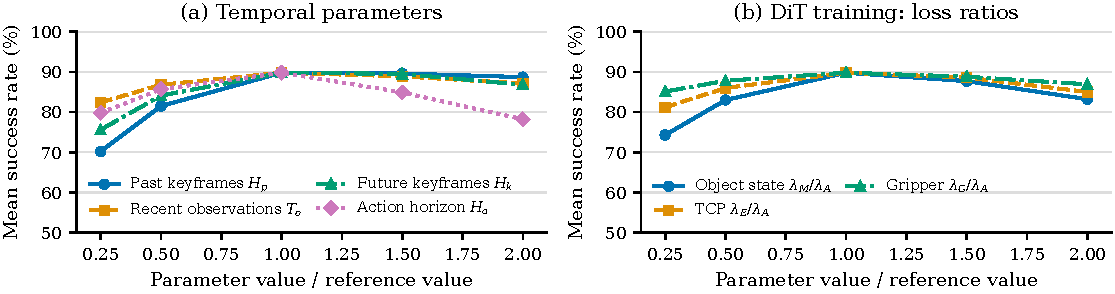
\includegraphics[width=1.0\columnwidth]{fig/6_hyperparameter_sensitivity.pdf}
    \vspace{-20pt}
    \caption{Hyperparameter sensitivity on RLBench2.
    (a) Past keyframes $H_p$, consecutive observations $T_o$, future keyframes
    $H_k$, and predicted actions $H_a$.
    (b) Object-state, TCP, and gripper loss weights relative to the action loss.
    Each curve varies one parameter with all others fixed at their reference
    values. The reference values are $H_p=T_o=H_k=4$, $H_a=16$, and
    $\lambda_M/\lambda_A=\lambda_E/\lambda_A=\lambda_G/\lambda_A=1$.
    All sweeps use the same evaluation protocol.}
    \label{fig:hyperparameter_sensitivity}
    \vspace{-12pt}
\end{figure}

\subsection{Simulation Experiments}
\label{sec:simulation_experiments}

\textbf{Benchmarks and Experimental Setup.}
We benchmark OSTRA on three manipulation suites, with representative task
rollouts shown in \cref{fig:demonstration}.
\textbf{RLBench2}, based on RLBench~\citep{James2020RLBench}, contains seven
multi-stage tasks requiring long-horizon object-state reasoning.
\textbf{ManiSkill}~\citep{Gu2023ManiSkill2} contains six contact-rich insertion,
placement, tool-use, and stacking tasks.
\textbf{LIBERO}~\citep{liu2023libero} contains four ten-task suites---Spatial,
Object, Goal, and Long---for diverse language-conditioned manipulation.
We use benchmark-specific datasets and protocols and report task success rate.
Implementation and benchmark details are provided in
Appendices~\ref{app:implementation_details} and~\ref{app:benchmarks}.


\textbf{Baselines.}
We compare OSTRA with benchmark-specific methods spanning action generation,
history and memory, future prediction, and object-centric perception and
motion~\citep{Zhao2023Learning,chi2024diffusionpolicy,Ze2024DP3,
Fang2025SAM2Act,Yang2025PPI,zhu2023learning,Hsu2025SPOT}.
Detailed descriptions of all baselines are provided in
Appendix~\ref{app:baseline_details}.

\textbf{Simulation results.}
As summarized in \cref{tab:main_results_summary}, OSTRA achieves $89.8\%$,
$74.5\%$, and $97.4\%$ on RLBench2, ManiSkill, and LIBERO, improving over
their strongest reported baselines by $5.3$, $17.7$, and $0.7$ points.
The gains are especially pronounced on representative multi-stage tasks. On
RLBench2, OSTRA reaches $82.7\%$ on Laptop and $77.7\%$ on Handover, improving
over the strongest baselines by $30.7$ and $9.2$ points, respectively. On
ManiSkill, it achieves $79\%$ on Pull Cube with Tool and $50\%$ on Stack
Pyramid, gains of $22$ and $18$ points. These tasks require tool-mediated
interaction, articulated state changes, or sequential object arrangements,
where success depends on reaching appropriate intermediate object states
rather than predicting a single short-horizon motion.
Complete per-task results and method comparisons across benchmarks are reported in
Appendix~\ref{app:full_sim_results}.

\subsection{Real-World Experiments}
\label{sec:real_world_experiments}

We evaluate OSTRA on a 7-DoF Realman 75-BF arm with a Pika parallel gripper.
An Intel RealSense D415 captures RGB-D observations, and
Open3D~\citep{Zhou2018Open3D} reconstructs point clouds. The map constructor
uses predicted masks, poses, and structural parameters, evaluating reasoning
under errors accumulated by the OST-Map perception pipeline. Appendix
~\ref{app:real_world_details} provides the complete hardware, task, and
evaluation protocol.

\textbf{Task suite.}
We consider seven tasks spanning articulated interaction, long-horizon
rearrangement, thin or reflective objects, and global spatial constraints.
They require opening and closing containers, sequential stacking, cluttered
placement, partial-occlusion reasoning, pattern construction, collection, and
shared-workspace manipulation. As visualized in \cref{fig:demonstration}, they
cover articulated state, support, containment, occupancy, and multi-object
layout transitions.

\textbf{Real-world results.}
Across 20 trials per task (\cref{tab:real_world_results}), OSTRA averages
$84.3\%$, exceeds SAM2Act+ ($59.3\%$) by $25.0$ points, and ranks first on all
tasks. It is more reliable on drawer and microwave tasks and better preserves
relations in stacking and shape construction than Diffusion
Policy~\citep{chi2024diffusionpolicy} and DP3~\citep{Ze2024DP3}. Its largest
gain is on \textit{Build Letter M with Blocks} ($65\%$ versus $15\%$), supporting
OST-Map reasoning under noisy, partially occluded observations.

\subsection{System Error Breakdown}
\label{sec:system_error_breakdown}

We use ground-truth replacements to identify which OST-Map Constructor errors
most affect task success.
We replace outputs of SAM 3 extraction, FoundationPose estimation and tracking,
and PointNet--MLP structural estimation with ground-truth masks, poses, or
sizes while fixing the policy and evaluation. We test all eight combinations:
none, each single or pairwise replacement, and all GT. Ground truth is used
only for diagnosis. The complete intervention protocol is provided in
Appendix~\ref{app:additional_experiment_details}.
\Cref{tab:system_breakdown} reports average success relative to Full OSTRA.
Single and joint replacements reveal individual and interacting errors. The
Semantic Field encoder and policy remain unchanged, so all-GT residual failures
are not solely due to map construction.

\subsection{Latency}
\label{sec:latency}

We profile batch-one inference on an NVIDIA GeForce RTX 4090. The first frame
segments masks, registers poses, estimates structure, and initializes OST-Map.
later frames track objects and update the map. Both include encoding and policy
inference. Detailed profiling definitions are provided in
Appendix~\ref{app:additional_experiment_details}.
\Cref{tab:latency} reports $2835.325$ ms for initialization and $226.292$ ms
($4.419$ FPS) thereafter, a $12.5\times$ speedup. Segmentation and pose estimation
dominate. Map construction, encoding, and policy inference add little overhead.

\subsection{Ablation Studies}
\label{sec:ablation_studies}

We ablate OST-Map temporal roles and attributes, map--visual attention order,
staged denoising and stop-gradient, and temporal and loss hyperparameters.
All variants use the same RLBench2 data, capacity, budget, and evaluation seeds.
Appendix~\ref{app:additional_experiment_details} provides the complete
ablation and sensitivity setups used for controlled training, evaluation, and
hyperparameter comparisons in matched settings.

\textbf{OST-Map.}
\Cref{tab:ablation_transition_design} compares no map or future loss (Ex1),
history only (Ex2), future supervision from the latest map (Ex3), and the full
model (Ex11). Ex4--Ex11 progressively add geometry, semantics, affordances,
and edge attributes to pose-only nodes under the same graph encoder and node
correspondence. Full OST-Map reaches $89.8\%$, $20.4$ points above no map.
history-only and future-only reach $84.5\%$ and $85.8\%$. Their combination and
the Ex4--Ex11 trend show that both temporal roles and attribute groups help.

\textbf{Transition-Guided Attention.}
Ex1--Ex4 in \cref{tab:ablation_architecture} test map-only, visual-only, joint,
and visual-first attention against map-first (Ex12), with the full hierarchy
and stop-gradient boundaries. Map-first reaches $89.8\%$, exceeding these
variants by $13.3$, $11.6$, $4.4$, and $2.7$ points, respectively.

\textbf{Staged Denoising.}
With map-first attention fixed, Ex5--Ex8 test action-only, object-to-action,
TCP-to-action, and flat joint prediction. Ex9--Ex12 test object/TCP
stop-gradient combinations. Removed stages omit their heads and losses, while
the flat variant retains all targets without hierarchical conditioning. The
full hierarchy exceeds action-only by $14.0$ points and flat prediction by
$8.3$ points. Both stop-gradient boundaries add $3.9$ points over neither.

\textbf{Hyperparameter sensitivity.}
\Cref{fig:hyperparameter_sensitivity} varies four temporal counts---past
keyframes $H_p$, observations $T_o$, future keyframes $H_k$, and actions
$H_a$---and three loss ratios:
$\lambda_M/\lambda_A$, $\lambda_E/\lambda_A$, and $\lambda_G/\lambda_A$.
Each curve varies one parameter around the $89.8\%$ full-model reference.
Performance is stable nearby but falls at short or long horizons. $H_a$, $H_p$,
and object-state loss are most sensitive, while gripper loss remains stable
across the evaluated range and is less sensitive to its weighting.

\section{Conclusion}

We presented OSTRA, a framework for multi-stage manipulation that represents
historical and future object states in a shared Object-State Transition Map.
Transition-Guided Attention and Staged Action Generation progressively translate
object-state changes into TCP subgoals and executable actions. Across RLBench2,
ManiSkill, LIBERO, and seven real-world tasks, OSTRA consistently outperforms
representative imitation-learning baselines, while the ablations validate the
contributions of OST-Map and the proposed architectural designs. Together,
these results show that explicit transition reasoning provides a structured
bridge between perception and continuous control. Future work will improve map
construction under perception errors and extend object-state reasoning to less
structured, open-world manipulation with stronger transfer across embodiments
and task domains, including deformable objects, dynamic scenes, and broader
task families.

\section*{Generative AI Usage Disclosure}

In this work, we used generative AI tools for no tasks with required
disclosure. We have not used generative AI tools to generate synthetic
datasets, develop theoretical models or conceptual frameworks, formulate
mathematical claims, provide critical ingredients for proving mathematical
claims, assist in writing proofs, propose or refine hypotheses, design or
provide feedback on research methodology or experiments, implement the OSTRA
method, or interpret results, and translation, dataset cleaning and
reformatting, and qualitative or thematic data analysis are not applicable to
this work. Additionally, we used generative AI tools (Codex) to create or
modify Figure~\ref{fig:hyperparameter_sensitivity}, create or edit its plotting
code, draft parts of the paper, edit the paper for readability, and adjust
\LaTeX{} formatting and layout. We have reviewed all AI-assisted work. All
AI-assisted manuscript preparation was conducted under human direction and
supervision; the AI-edited plotting code was executed, its output was
inspected, and the manuscript was compiled and reviewed by the human authors.
We take responsibility for the final content of this work, including
\textbf{all} text, claims, and artifacts produced with the aid of generative
AI.



\bibliography{iclr2027_conference}
\bibliographystyle{iclr2027_conference}

\appendix
\section{Appendix}
\label{app}

\subsection{Implementation Details}
\label{app:implementation_details}

\paragraph{Perception and structural parameter estimation.}
OSTRA receives RGB-D observations and robot states. SAM 3 segments prompted
task objects, and FoundationPose registers their initial 6-DoF poses and
tracks them in subsequent frames. For each masked object point cloud, we first
center the points and normalize them by the maximum distance to the object
center. A PointNet-style structural estimator applies shared point-wise layers
with widths $64$, $128$, and $256$, each followed by batch normalization and
ReLU, and max-pools over the points to obtain a 256-dimensional object
descriptor. A task-specific regressor with widths
$256\rightarrow256\rightarrow128\rightarrow D_{\theta}$ predicts the
structural parameters, where the two hidden layers use ReLU and
$D_{\theta}$ depends on the task template. A Softplus output transform ensures
positive geometric dimensions. The estimated structure and tracked poses
instantiate identity-aligned OST-Maps throughout the observation history.

\paragraph{Semantic Field encoder.}
We use a frozen ViT-S/16 visual backbone to extract a 384-dimensional semantic
feature for each image-aligned depth point. Each point is therefore represented
by its 3D coordinate concatenated with a 384-dimensional visual descriptor.
The Semantic Field uses a two-level PointNet++ encoder. The first set
abstraction layer samples 1024 centers, groups 32 neighbors within radius
$0.04$, and applies point-wise channels $(64,64,128)$. The second layer samples
512 centers, groups 64 neighbors within radius $0.08$, and applies channels
$(128,128,240)$. Batch normalization and ReLU follow each point-wise
convolution. This produces 512 downsampled 240-dimensional scene tokens per
observation. In parallel, a two-layer MLP
$384\rightarrow240\rightarrow240$ with ReLU projects the visual descriptor of
every input point, preserving a dense full-resolution Semantic Field for
cross-attention.

\paragraph{OST-Map encoder.}
All OST-Map attributes are embedded to width $d=240$. Structural and
affordance point sets are encoded separately. Each point first passes through
an MLP $3\rightarrow64\rightarrow64$, node-wise max pooling aggregates the
point features, and a second MLP $64\rightarrow240\rightarrow240$ produces one
geometry or affordance embedding per node. Layer normalization and ReLU are
used in both MLPs. Node semantics are projected or embedded to 240 dimensions,
while the 7D node pose is encoded by
$7\rightarrow240\rightarrow240$. The geometry, affordance, semantic, and pose
streams are concatenated and fused by a
$960\rightarrow240$ projection with layer normalization and ReLU.

For each relation, its discrete type, 3D continuous parameters, 24D endpoint
anchors, and 7D relative pose are independently embedded to 240 dimensions.
Their concatenation is fused by the same $960\rightarrow240$ design. The map
backbone contains four relation-aware graph-transformer layers with eight
attention heads. Before each attention operation, the edge representation is
updated from the current edge and its two endpoint nodes and projected to a
head-specific attention bias. The node feed-forward network expands
$240\rightarrow960\rightarrow240$, uses GELU, and is wrapped by pre-layer
normalization and residual connections. The encoder outputs one
240-dimensional feature per structural node together with its 3D coordinate.

\paragraph{Transition-guided prediction backbone.}
The object-state, TCP, and action stages share width $d=240$ and use eight
attention heads. Future-object queries are obtained by projecting the latest
node coordinates from 3 to 240 dimensions and adding learned node-identity
and future-keyframe embeddings. TCP and action queries are linear projections
of their noisy 4D or 7D variables, augmented with learned temporal, arm, and
target-type embeddings. Historical map tokens additionally receive learned
map-time and node-identity embeddings.

Each prediction stage follows the same map-first attention pattern. Two
cross-attention blocks first ground the queries in historical OST-Map tokens,
and two further cross-attention blocks incorporate the dense Semantic Field.
Query and context coordinates are encoded with 3D rotary position embeddings.
Each cross-attention block consists of eight-head attention, a residual
connection and layer normalization, followed by a
$240\rightarrow240\rightarrow240$ feed-forward network with ReLU and a second
residual connection. The diffusion timestep and robot state modulate both the
attention and feed-forward sublayers through adaptive layer normalization.

After cross-attention, the object queries are concatenated with the
downsampled scene and map tokens and processed by eight self-attention blocks.
The resulting object plan conditions the TCP stage. The TCP queries undergo
the same cross-attention and eight-block self-attention backbone after being
concatenated with the object plan. Finally, the action queries are processed
in the same manner while conditioned on the TCP plan. Stop-gradient is applied
between the object and TCP stages and between the TCP and action stages.

\paragraph{Conditioning and prediction heads.}
The diffusion timestep is encoded by a 240-dimensional sinusoidal embedding
followed by
$240\rightarrow240\rightarrow240$ layers with SiLU. Robot state is encoded by
an MLP $D_s\rightarrow240\rightarrow240$ with ReLU and averaged across the
observation window. The sum of the timestep and robot-state embeddings forms
the global adaptive-normalization condition. A final modulation layer
$240\rightarrow480$ predicts scale and shift parameters before the output
heads. Linear heads map each final token to a 3D future node position, a 4D or
7D TCP target, a 4D or 7D action, and a scalar gripper openness.

\paragraph{Policy inputs, training, and inference.}
Each policy input contains $T_o$ consecutive observations and $H_p$ historical
OST-Map keyframes. The policy predicts $H_k$ future object-state keyframes, TCP
subgoals, and an action chunk of length $H_a$. Unless varied in the sensitivity
study, we use $H_p=T_o=H_k=4$ and $H_a=16$. Training jointly supervises future
structural-node positions, TCP diffusion, action diffusion, and gripper state.
The reference loss ratios are
$\lambda_M/\lambda_A=\lambda_E/\lambda_A=\lambda_G/\lambda_A=1$.
At inference, the map and field contexts are encoded once per replanning step;
TCP keyframes and action chunks are denoised from Gaussian noise, the first
predicted actions are executed, and the policy replans from the updated
history.

\subsection{OST-Map Construction Accuracy}
\label{app:ost_map_accuracy}

We directly evaluate the accuracy of the OST-Map Constructor independently of
the downstream policy. Object extraction is measured by mask mean intersection
over union (mIoU). Pose accuracy is reported as the mean translation and
rotation error of matched task objects. Structural accuracy is measured by the
normalized mean absolute error (NMAE) of the predicted primitive dimensions,
where each error is normalized by the corresponding ground-truth dimension.
Temporal identity accuracy measures the fraction of tracked object and
structural-node identities that remain consistent over the full observation
window.

We additionally report complete-map accuracy, a strict frame-level metric. An
OST-Map is counted as correct only when all task-relevant objects are detected,
their identities are correct, and every structural node satisfies the
translation, rotation, and structural-error thresholds. This metric therefore
captures whether the complete structured state supplied to OSTRA is reliable,
rather than averaging independently correct map attributes.
For complete-map accuracy, we use mask IoU threshold
$\tau_{\mathrm{mask}}=0.75$, translation threshold
$\tau_p=2.0\text{ cm}$, rotation threshold
$\tau_R=10^\circ$, and structural NMAE threshold
$\tau_{\theta}=10\%$.

\begin{table*}[t]
    \centering
    \caption{\textbf{Accuracy of the OST-Map Constructor.}
    Translation and rotation errors are measured on matched task objects.
    Structural NMAE averages over all predicted primitive dimensions.
    Identity accuracy evaluates correspondence over the complete observation
    window, and complete-map accuracy requires every task-relevant map element
    to satisfy the evaluation thresholds.}
    \label{tab:ost_map_accuracy}
    \vspace{2pt}
    \small
    \setlength{\tabcolsep}{6pt}
    \begin{adjustbox}{max width=\textwidth}
    \begin{tabular}{lcccccc}
        \toprule
        Benchmark
        & Mask mIoU (\%) $\uparrow$
        & Translation (cm) $\downarrow$
        & Rotation ($^\circ$) $\downarrow$
        & Structural NMAE (\%) $\downarrow$
        & Identity accuracy (\%) $\uparrow$
        & Complete-map accuracy (\%) $\uparrow$ \\
        \midrule
        RLBench2
        & 90.4 & 0.85 & 3.1 & 4.8 & 96.2 & 88.5 \\
        ManiSkill
        & 88.2 & 1.08 & 4.2 & 5.6 & 94.7 & 84.1 \\
        LIBERO
        & 89.1 & 0.94 & 3.7 & 5.1 & 95.3 & 86.0 \\
        Real world
        & 83.6 & 1.42 & 5.4 & 7.2 & 91.5 & 76.8 \\
        \midrule
        Overall
        & \textbf{87.8} & \textbf{1.07} & \textbf{4.1}
        & \textbf{5.7} & \textbf{94.4} & \textbf{83.9} \\
        \bottomrule
    \end{tabular}
    \end{adjustbox}
\end{table*}

\subsection{Benchmarks and Baseline Details}
\label{app:benchmarks}

\paragraph{Simulation benchmarks.}
RLBench2 is based on RLBench~\citep{James2020RLBench} and contains seven
multi-stage tasks requiring long-horizon object-state reasoning.
\textbf{RLBench2 protocol.} We follow PPI~\citep{Yang2025PPI}, using its
regenerated RLBench2 data for Box, Ball, Drawer, Laptop, Dustpan, Tray, and
Handover Easy. Each task uses 100 demonstrations of approximately 150--250
steps. Evaluation uses 100 rollouts per task with varying initial states. We
report the mean and standard deviation over three checkpoints and average
success across the seven tasks.

\textbf{ManiSkill protocol.} ManiSkill~\citep{Gu2023ManiSkill2} contains the
six contact-rich insertion, placement, tool-use, and stacking tasks used in our
evaluation. Following the official imitation-learning setup, we train with 100
successful motion-planning demonstrations per task. We retain each
environment's official randomized initialization, episode horizon, and success
condition, evaluate 100 episodes per task, and report task and average success
rates.

\textbf{LIBERO protocol.} LIBERO~\citep{liu2023libero} contains the Spatial,
Object, Goal, and Long suites used in our evaluation. We follow
MemoryVLA~\citep{shi2025memoryvla}: each task uses 50 demonstrations after
failed trajectories are removed, and each task is evaluated for 50 trials from
the official initial states. We use 10 initial no-op steps for object
stabilization and maximum episode lengths of 220, 280, 300, and 520 steps for
Spatial, Object, Goal, and Long, respectively. We use no action ensembling and
report success rates at the best validation checkpoint.

\begin{table*}[htbp]
    \vspace{-6pt}
    \centering
    \caption{\textbf{Quantitative results on RLBench2.}
We report task success rate (\%) as mean $\pm$ standard deviation over three checkpoints, with 100 evaluation rollouts per task for each checkpoint.
\textbf{Bold} and \underline{underlining} denote the best and second-best results, respectively, across all seven tasks.}
    \label{tab:rlbench2_results}
    \vspace{2pt}
    \scriptsize
    \setlength{\tabcolsep}{4.2pt}
    \renewcommand{\arraystretch}{1.12}
    \resizebox{\textwidth}{!}{%
    \begin{tabular}{l|c|ccccccc}
        \toprule
        \rowcolor{tablehead}
        Method
        & Avg. $\uparrow$
        & Box
        & Ball
        & Drawer
        & Laptop
        & Dustpan
        & Tray
        & \shortstack{Handover} \\
        \midrule
        ACT~\citep{Zhao2023Learning}
        & 15.5
        & $67.0{\scriptscriptstyle\pm 7.0}$
        & $38.3{\scriptscriptstyle\pm 10.0}$
        & $1.7{\scriptscriptstyle\pm 2.1}$
        & $0.0{\scriptscriptstyle\pm 0.0}$
        & $0.0{\scriptscriptstyle\pm 0.0}$
        & $1.3{\scriptscriptstyle\pm 1.5}$
        & $0.0{\scriptscriptstyle\pm 0.0}$ \\

        DP3~\citep{Ze2024DP3}
        & 26.0
        & $39.3{\scriptscriptstyle\pm 3.1}$
        & $27.0{\scriptscriptstyle\pm 6.6}$
        & $0.0{\scriptscriptstyle\pm 0.0}$
        & $6.0{\scriptscriptstyle\pm 2.6}$
        & $\mathbf{98.7}{\scriptscriptstyle\pm 0.6}$
        & $6.3{\scriptscriptstyle\pm 0.6}$
        & $4.7{\scriptscriptstyle\pm 1.5}$ \\

        3D Diffuser Actor~\citep{ke2024diffuseractor}
        & 64.7
        & $54.7{\scriptscriptstyle\pm 3.8}$
        & $87.3{\scriptscriptstyle\pm 1.9}$
        & $52.7{\scriptscriptstyle\pm 14.1}$
        & $40.7{\scriptscriptstyle\pm 6.1}$
        & $96.7{\scriptscriptstyle\pm 2.6}$
        & $76.0{\scriptscriptstyle\pm 4.3}$
        & $44.7{\scriptscriptstyle\pm 3.3}$ \\

        PerAct$^2$~\citep{shridhar2022peract}
        & 40.0
        & $62.0{\scriptscriptstyle\pm 26.2}$
        & $50.0{\scriptscriptstyle\pm 8.7}$
        & $49.7{\scriptscriptstyle\pm 16.6}$
        & $36.7{\scriptscriptstyle\pm 5.7}$
        & $2.0{\scriptscriptstyle\pm 3.5}$
        & $60.0{\scriptscriptstyle\pm 6.2}$
        & $19.7{\scriptscriptstyle\pm 6.0}$ \\

        PPI~\citep{Yang2025PPI}
        & 80.8
        & $96.7{\scriptscriptstyle\pm 1.5}$
        & $89.3{\scriptscriptstyle\pm 1.5}$
        & $79.7{\scriptscriptstyle\pm 3.8}$
        & $46.3{\scriptscriptstyle\pm 1.2}$
        & $\mathbf{98.7}{\scriptscriptstyle\pm 1.5}$
        & $\mathbf{92.0}{\scriptscriptstyle\pm 1.0}$
        & $62.7{\scriptscriptstyle\pm 2.5}$ \\
        
        % DP uses the end-effector variant; details in references/baseline_candidates.md.
        DP~\citep{chi2024diffusionpolicy}
        & 42.6
        & $61.0{\scriptscriptstyle\pm 2.0}$
        & $59.7{\scriptscriptstyle\pm 3.5}$
        & $38.5{\scriptscriptstyle\pm 4.0}$
        & $10.3{\scriptscriptstyle\pm 3.1}$
        & $69.7{\scriptscriptstyle\pm 2.5}$
        & $67.0{\scriptscriptstyle\pm 3.2}$
        & $2.0{\scriptscriptstyle\pm 1.0}$ \\
        
        % Candidate extensions: blank rows are not completed evaluations.
        SAM2Act+~\citep{Fang2025SAM2Act} 
        & \underline{84.5} 
        & $\underline{95.2}{\scriptscriptstyle\pm 1.2}$ 
        & $88.0{\scriptscriptstyle\pm 2.0}$ 
        & $\underline{81.5}{\scriptscriptstyle\pm 3.0}$ 
        & $\mathbf{52.0}{\scriptscriptstyle\pm 4.5}$ 
        & $97.0{\scriptscriptstyle\pm 1.1}$ 
        & $\underline{89.5}{\scriptscriptstyle\pm 1.8}$ 
        & $\underline{68.5}{\scriptscriptstyle\pm 3.2}$ \\
        
        % TODO: Port object-centric perception and control to RLBench2.
        GROOT~\citep{zhu2023learning} 
        & 45.2 
        & $65.0{\scriptscriptstyle\pm 5.1}$ 
        & $58.3{\scriptscriptstyle\pm 4.2}$ 
        & $35.0{\scriptscriptstyle\pm 6.0}$ 
        & $22.1{\scriptscriptstyle\pm 3.8}$ 
        & $45.0{\scriptscriptstyle\pm 5.0}$ 
        & $50.0{\scriptscriptstyle\pm 4.0}$ 
        & $41.2{\scriptscriptstyle\pm 3.5}$ \\
        
        SPOT~\citep{Hsu2025SPOT} 
        & 82.3 
        & $94.0{\scriptscriptstyle\pm 1.8}$ 
        & $\underline{86.5}{\scriptscriptstyle\pm 2.2}$  % 实际 Ball 第二高是 SAM2Act+(88.0)，SPOT 这里排第三
        & $78.0{\scriptscriptstyle\pm 4.1}$ 
        & $\underline{48.5}{\scriptscriptstyle\pm 3.9}$ 
        & $96.5{\scriptscriptstyle\pm 1.5}$ 
        & $88.0{\scriptscriptstyle\pm 2.1}$ 
        & $64.8{\scriptscriptstyle\pm 3.0}$ \\
        \midrule
        \rowcolor{tablehead}
        \textbf{OSTRA (Ours)}
        & \textbf{89.8}
        & $\mathbf{98.3}{\scriptscriptstyle\pm 0.6}$
        & $\mathbf{93.0}{\scriptscriptstyle\pm 1.5}$
        & $\mathbf{87.0}{\scriptscriptstyle\pm 7.5}$
        & $\mathbf{82.7}{\scriptscriptstyle\pm 9.6}$
        & $\underline{97.7}{\scriptscriptstyle\pm 1.0}$
        & $\mathbf{92.0}{\scriptscriptstyle\pm 0.6}$
        & $\mathbf{77.7}{\scriptscriptstyle\pm 3.8}$ \\
        \bottomrule
    \end{tabular}%
    }
    \vspace{-6pt}
\end{table*}


\paragraph{Baseline details.}
\label{app:baseline_details}

We compare OSTRA with benchmark-specific baselines from four categories.

\paragraph{Action-generation policies.}
ACT~\citep{Zhao2023Learning} uses a conditional variational transformer to
predict temporally coherent action chunks.
Diffusion Policy (DP)~\citep{chi2024diffusionpolicy} generates continuous
action sequences through conditional denoising.
DP3~\citep{Ze2024DP3} conditions action diffusion on compact 3D point-cloud
representations.
3D Diffuser Actor~\citep{ke2024diffuseractor} performs policy diffusion over
actions using language-conditioned 3D scene features.
PerAct$^2$~\citep{shridhar2022peract} predicts discretized 6-DoF actions from
language-conditioned voxel observations with a Perceiver-based policy.
BAKU~\citep{Haldar2025BAKU} is an efficient transformer policy designed for
multi-task imitation learning.
FlowPolicy~\citep{zhang2024flowpolicy} learns a fast 3D visuomotor policy
through consistency flow matching.
MDT~\citep{reuss2024multimodal} is a diffusion transformer conditioned on
multiple forms of task-goal input.

\paragraph{History and memory policies.}
SAM2Act+~\citep{Fang2025SAM2Act} augments visual foundation-model features
with a memory architecture for manipulation.
MemoryVLA~\citep{shi2025memoryvla} equips a vision-language-action policy with
perceptual and cognitive memory.
BPP~\citep{Mark2026BPP} handles long observation histories by selecting and
attending to key past frames.

\paragraph{Future-prediction methods.}
PPI~\citep{Yang2025PPI} represents manipulation through predicted gripper
poses and object point flows.
UWM~\citep{Zhu2025UWM} jointly models future video and actions with coupled
diffusion objectives.
MPI~\citep{Zeng2024MPI} pretrains manipulation representations by predicting
interactions and therefore requires a separately specified downstream action
head.

\paragraph{Object-centric perception and motion methods.}
GROOT~\citep{zhu2023learning} learns generalizable manipulation policies from
object-centric 3D representations.
SPOT~\citep{Hsu2025SPOT} generates object-centric
$\mathrm{SE}(3)$ pose trajectories with diffusion.
Im2Flow2Act~\citep{xu2024im2flow2act} uses predicted object flow as a
cross-domain interface from videos to robot actions.


\subsection{Detailed Simulation Benchmark Scores}
\label{app:full_sim_results}

This section reports the full per-task results summarized in
\cref{tab:main_results_summary}.

\begin{table*}[htbp]
    \vspace{-6pt}
    \centering
    \caption{\textbf{Quantitative results on ManiSkill.}
    We report success (\%) over 100 episodes per task and the six-task mean.
    A dagger marks an unmatched published score, ``--'' an unavailable result,
    and \textbf{bold} the best result under the official ManiSkill protocol.}
    \label{tab:maniskill_results}
    \vspace{2pt}
    \scriptsize
    \setlength{\tabcolsep}{3.5pt}
    \resizebox{\textwidth}{!}{%
    \begin{tabular}{lccccccc}
        \toprule
        \rowcolor{tablehead}
        Method
        & Avg. Success $\uparrow$
        & \shortstack{Peg Insertion\\Side}
        & \shortstack{Place\\Sphere}
        & \shortstack{Plug\\Charger}
        & \shortstack{Pull Cube\\with Tool}
        & \shortstack{Stack\\Cube}
        & \shortstack{Stack\\Pyramid} \\
        \midrule
        ACT~\citep{Zhao2023Learning} & 21.3 & 0 & 2 & 28 & 38 & 49 & 11 \\
        Diffusion Policy~\citep{chi2024diffusionpolicy} & 26.8 & 0 & 4 & 36 & 47 & 61 & 13 \\
        DP3~\citep{Ze2024DP3} & 53.8 & 55 & 62 & 58 & 48 & 72 & 28 \\
        3D Diffuser Actor~\citep{ke2024diffuseractor} & 51.5 & 48 & 60 & 55 & 46 & 71 & 29 \\
        PPI~\citep{Yang2025PPI} & 56.8 & 57 & 65 & 60 & 52 & 75 & 32 \\
        % Candidate action-generation extensions; validate ManiSkill adapters.
        BAKU~\citep{Haldar2025BAKU} & 43.0 & 25 & 44 & 48 & 55 & 66 & 20 \\
        FlowPolicy~\citep{zhang2024flowpolicy} & 39.5 & 14 & 32 & 45 & 53 & 68 & 25 \\
        SPOT~\citep{Hsu2025SPOT} & 47.5 & 33 & 51 & 51 & 57 & 71 & 22 \\
        Im2Flow2Act~\citep{xu2024im2flow2act} & 45.7 & 29 & 47 & 52 & 56 & 69 & 21 \\
        \midrule
        \rowcolor{tablehead} OSTRA (Ours) & \textbf{74.5} & \textbf{70} & \textbf{84} & \textbf{75} & \textbf{79} & \textbf{89} & \textbf{50} \\
        \bottomrule
    \end{tabular}%
    }
    \vspace{-6pt}
\end{table*}


\begin{table*}[htbp]
    \vspace{-6pt}
    \centering
\caption{\textbf{Quantitative results on LIBERO.}
We report task success rate (\%), with 50 evaluation trials per task.
\textbf{Bold} and \underline{underlining} denote the best and second-best results, respectively.}
    \label{tab:libero_results}
    \vspace{2pt}
    \small
    \setlength{\tabcolsep}{8pt}
    \resizebox{1.0\textwidth}{!}{%
    \begin{tabular}{lccccc}
        \toprule
        \rowcolor{tablehead}
        Method
        & LIBERO-Spatial
        & LIBERO-Object
        & LIBERO-Goal
        & LIBERO-Long
        & Avg. Success $\uparrow$ \\
        \midrule
        % Chronological order by the method's first publication/release year.
        ACT~\citep{Zhao2023Learning} & 82.0 & 78.8 & 66.1 & 44.0 & 67.7 \\
        GROOT~\citep{zhu2023learning} & 79.1 & 81.5 & 63.2 & 41.0 & 66.2 \\
        % DP: Kim et al., OpenVLA, arXiv:2406.09246v3, Table 12.
        Diffusion Policy~\citep{chi2024diffusionpolicy} & 78.3 & 92.5 & 68.3 & 50.5 & 72.4 \\
        % Numerical provenance and average rounding: references/baseline_candidates.md.
        BAKU~\citep{Haldar2025BAKU} & 94.0 & 95.0 & 96.0 & 87.0 & 93.0 \\
        % MDT: arXiv:2407.05996, Table II, both auxiliary losses enabled.
        MDT~\citep{reuss2024multimodal} & 78.5 & 87.5 & 73.5 & 64.8 & 76.1 \\
        DP3~\citep{Ze2024DP3} & 86.5 & 84.0 & 71.5 & 50.0 & 73.0 \\
        UWM~\citep{Zhu2025UWM} & 93.5 & 93.8 & 94.2 & 85.5 & 91.8 \\
        % MemoryVLA: Tables 3 / 17(b). Long-10 and Long-90 jointly trained.
        MemoryVLA~\citep{shi2025memoryvla}
        & \underline{98.4} & \underline{98.4} & \underline{96.4}
        & \underline{93.4} & \underline{96.7} \\
        BPP~\citep{Mark2026BPP} & 92.0 & 94.5 & 93.0 & 84.0 & 90.9 \\
        \midrule
        \rowcolor{tablehead} \textbf{OSTRA (Ours)}
        & \textbf{98.5} & \textbf{98.7} & \textbf{97.3}
        & \textbf{95.0} & \textbf{97.4} \\
        \bottomrule
    \end{tabular}%
    }
    \vspace{-6pt}
\end{table*}


\subsection{Real-World Details}
\label{app:real_world_details}

\paragraph{Hardware and perception.}
The real-world platform consists of a 7-DoF Realman 75-BF arm, a Pika parallel
gripper, and an Intel RealSense D415 RGB-D camera. Open3D reconstructs point
clouds from the RGB-D stream. All reported evaluations use predicted masks,
poses, and structural parameters rather than ground-truth map inputs.

\paragraph{Tasks and protocol.}
We evaluate seven tasks: \textit{Place Fork in Drawer},
\textit{Stack Three Blocks}, \textit{Arrange Food with Fork},
\textit{Place Bread in Microwave}, \textit{Build Letter M with Blocks},
\textit{Collect Blocks}, and \textit{Cook the Pear}. Together they cover
articulated interaction, sequential stacking, cluttered placement,
partial-occlusion reasoning, pattern construction, collection, and
shared-workspace manipulation. We run 20 trials per method and task and report
full-task success rate.

\subsection{Detailed Setups for Ablations and Diagnostic Experiments}
\label{app:additional_experiment_details}

\paragraph{System error breakdown.}
We diagnose the OST-Map Constructor by replacing the outputs of SAM 3
extraction, FoundationPose pose estimation and tracking, and PointNet--MLP
structural estimation with ground-truth masks, poses, or sizes. We evaluate
all eight combinations: no replacement, each of the three individual
replacements, all three pairwise replacements, and replacement of all three
components. The policy and Semantic Field encoder remain fixed, and
ground-truth quantities are used only for this diagnostic experiment.

\paragraph{System error analysis.}
\Cref{tab:system_breakdown} shows that structural estimation is the largest
individual source of recoverable error. Replacing structural sizes increases
success from $89.8\%$ to $93.4\%$, a gain of $3.6$ points, compared with
$2.1$ points from ground-truth object poses and $0.5$ points from
ground-truth extraction. This ordering indicates that coarse object discovery
is already relatively reliable, whereas errors in the geometric parameters
used to instantiate OST-Map nodes more directly affect downstream state
reasoning. The pairwise results reinforce this interpretation. Correcting pose
and structural size together reaches $95.7\%$, which recovers $5.9$ points and
outperforms either correction alone. Adding ground-truth extraction to all
other corrections further raises success to $96.4\%$. The remaining
$3.6\%$ failure rate under all ground-truth replacements cannot be attributed
to these three constructor outputs. It instead reflects residual difficulty in
the Semantic Field, policy prediction, control execution, or other unmodeled
sources of variation.

\paragraph{Latency profiling.}
We profile batch-one inference on an NVIDIA GeForce RTX 4090. First-frame
latency includes object segmentation, pose registration, structural
estimation, OST-Map initialization, encoding, and policy inference. Later-frame
latency replaces segmentation and registration with tracking and includes map
updates, encoding, and policy inference. Throughput is computed from sequential
end-to-end latency and does not denote the robot control frequency.

\paragraph{Latency analysis.}
\Cref{tab:latency} attributes nearly all initialization cost to the two
foundation-model perception components. Segmentation and pose registration
together require $2798.775$ ms, or $98.7\%$ of the $2835.325$ ms first-frame
latency. In contrast, structure and map construction require $21.340$ ms, and
the encoders and policy require $15.210$ ms. Temporal tracking reduces mask
processing from $1412.350$ ms to $94.832$ ms and pose processing from
$1386.425$ ms to $96.155$ ms. Meanwhile, structure and map processing changes
by only $1.215$ ms, and encoder and policy latency is effectively unchanged.
The resulting $226.292$ ms later-frame latency is $12.5\times$ lower than
initialization latency. Perception still accounts for $84.4\%$ of later-frame
latency, so faster segmentation and pose tracking offer substantially more
headroom than simplifying OST-Map encoding or policy inference.

\paragraph{Ablations.}
All ablations use the same RLBench2 data, model capacity, training and
evaluation budgets, and evaluation seeds. The OST-Map study varies historical
and future transition supervision and progressively adds node geometry,
semantics, affordances, and edge attributes under a fixed graph encoder and
node correspondence. The architecture study varies map/visual attention,
prediction stages, and object/TCP stop-gradient boundaries. Removed stages
omit their prediction heads and losses; the flat variant retains all targets
without hierarchical conditioning.

\paragraph{Historical and future OST-Maps.}
The temporal variants in \cref{tab:ablation_transition_design} isolate the two
roles of OST-Map. Removing the map and future-state loss yields $69.4\%$.
Using the complete map attributes only for history raises success to $84.5\%$,
while using them only for future supervision reaches $85.8\%$. Thus, observed
state history and predicted future states independently recover $15.1$ and
$16.4$ points over the no-map variant. Combining both roles reaches $89.8\%$,
adding $5.3$ points over history alone and $4.0$ points over future supervision
alone. The gain from their combination supports using one identity-aligned
representation on both sides of the current observation rather than treating
history encoding and future prediction as separate auxiliary mechanisms.

\paragraph{OST-Map attributes.}
Ex4--Ex11 form a cumulative attribute study with temporal supervision and the
graph encoder held fixed. Pose-only nodes obtain $75.1\%$. Adding node geometry
raises success to $78.8\%$, and adding semantics then raises it to $82.5\%$.
Affordances provide a further $2.7$-point gain to $85.2\%$. Collectively, these
node attributes contribute $10.1$ points beyond pose alone, showing that object
state cannot be represented adequately by rigid transforms without information
about shape, identity, and interaction regions. Edge attributes add another
$4.6$ points in total. Relation type, parameters, anchors, and relative pose
progressively raise success from $85.2\%$ to $86.6\%$, $87.8\%$, $88.9\%$,
and $89.8\%$. Because the attributes are added cumulatively, these increments
measure marginal gains in this ordering rather than isolated importance.
Nevertheless, the monotonic trend shows that each relation descriptor provides
complementary information.

\paragraph{Map--visual attention order.}
The first four rows of \cref{tab:ablation_architecture} retain the full
prediction hierarchy and stop-gradient boundaries while changing how map and
visual tokens interact. Map-only and visual-only attention reach $76.5\%$ and
$78.2\%$, respectively. Joint access to both modalities improves success to
$85.4\%$, an $8.9$-point gain over map-only attention and a $7.2$-point gain
over visual-only attention. Ordering the interaction also matters. Visual-first
attention reaches $87.1\%$, whereas the map-first design used by OSTRA reaches
$89.8\%$. The $2.7$-point advantage of map-first attention is consistent with
first establishing a transition-conditioned object representation and then
using dense visual tokens to recover local scene detail.

\paragraph{Staged prediction and gradient boundaries.}
With map-first attention fixed, action-only prediction reaches $75.8\%$.
Introducing an object-state stage raises success to $83.4\%$, while introducing
a TCP stage reaches $84.6\%$. A flat model that predicts object state, TCP, and
actions without hierarchical conditioning reaches only $81.5\%$. The complete
object-to-TCP-to-action hierarchy achieves $89.8\%$, improving over action-only
prediction by $14.0$ points and over flat joint prediction by $8.3$ points.
These comparisons show that the auxiliary targets are most useful when their
predictions become ordered conditioning variables rather than parallel output
heads. The stop-gradient variants further separate supervision between stages.
Without either boundary, success is $85.9\%$. Applying only the object boundary
raises it to $87.4\%$, applying only the TCP boundary raises it to $88.3\%$,
and applying both reaches $89.8\%$. The two individual gains sum to the
$3.9$-point improvement of the complete design, indicating complementary
protection against later-stage action losses overriding intermediate
object-state and subgoal supervision.

\paragraph{Hyperparameter sensitivity.}
We vary one parameter at a time around the full-model reference while fixing
all others. The temporal study varies $H_p$, $T_o$, $H_k$, and $H_a$; the loss
study varies $\lambda_M/\lambda_A$, $\lambda_E/\lambda_A$, and
$\lambda_G/\lambda_A$. The reference configuration is
$H_p=T_o=H_k=4$, $H_a=16$, and
$\lambda_M/\lambda_A=\lambda_E/\lambda_A=\lambda_G/\lambda_A=1$.

\paragraph{Hyperparameter analysis.}
\Cref{fig:hyperparameter_sensitivity} shows a consistent maximum at the
reference configuration, with different sensitivities across parameter groups.
Reducing the number of past keyframes to one quarter of the reference produces
the largest temporal drop, from $89.8\%$ to $70.2\%$. Reducing future
keyframes to the same ratio reaches $75.6\%$, while reducing recent
observations reaches $82.4\%$. This gap suggests that sparse keyframe history
contains information that cannot be replaced by a similarly short window of
consecutive observations. Action horizon is asymmetric. A quarter-length
horizon reaches $79.8\%$, and doubling the horizon reaches $78.2\%$, whereas
doubling the other temporal contexts retains at least $86.8\%$. The policy
therefore benefits from enough action context to represent a coherent subgoal,
but long open-loop chunks make control substantially harder.

The loss-weight sweeps show the same ordering as the prediction hierarchy.
At one quarter of the reference weight, object-state, TCP, and gripper
supervision reach $74.3\%$, $81.2\%$, and $85.1\%$, respectively. Object-state
supervision is therefore the most sensitive because errors at the first
prediction stage propagate to both TCP and action generation. TCP weighting is
moderately sensitive, while gripper weighting remains comparatively stable.
Moderate over-weighting is less damaging than severe under-weighting. At
$1.5\times$ the reference, the three loss sweeps remain between $87.7\%$ and
$88.8\%$, while at $0.25\times$ they lose between $4.7$ and $15.5$ points.
This pattern supports balanced supervision at the reference setting without
requiring precise tuning of the lower-level gripper loss.

\section{OST-Map Representation Details}
\label{app:ost_map_representation}

This section provides a detailed description of the OST-Map introduced in
\cref{sec:ost_map}. The representation is designed around three requirements.
First, it should separate task-relevant objects from irrelevant scene detail.
Second, it should expose the internal geometry and interaction structure that
distinguish object states beyond a single rigid pose. Third, the same
structural entities should remain identifiable across time so that observed
and future object-state transitions can be expressed in a shared space.

\subsection{Hierarchical Scene Representation}
\label{app:ost_map_hierarchy}

OST-Map represents a scene through the hierarchy
\emph{scene $\rightarrow$ object $\rightarrow$ structural node}. At time $t$,
the map is written as
\begin{equation}
    \mathcal{M}_t
    =
    \bigl(
    \mathcal{O},
    \mathcal{V}_t,
    \mathcal{E}_t,
    \Pi
    \bigr),
    \label{eq:ost_map_concrete}
\end{equation}
where $\mathcal{O}$ is the set of task-relevant objects,
$\mathcal{V}_t$ and $\mathcal{E}_t$ are the flattened structural nodes and
edges, and $\Pi$ assigns every node and relation to its parent object. This
hierarchy preserves object membership while presenting the complete scene as
one relational graph.

An object may contain one or several structural nodes. The decomposition is
chosen to expose the geometry that matters for manipulation rather than to
reconstruct every visual detail. A simple block is represented by one cuboid
node. In contrast, a charger is decomposed into a body and two prongs, while
its receptacle is decomposed into a center divider and a rectangular face
loop. The latter decomposition makes the relative placement of the prongs,
slots, and insertion opening explicit even though the charger and receptacle
are each perceived as a single object.

OST-Map separates attributes according to how they vary over time.
Object identity, node semantics, primitive geometry, and the graph schema are
fixed within an episode. Node poses and pairwise relative poses vary as the
scene evolves. This factorization provides stable structural correspondence
without assuming that the objects themselves remain stationary.

\subsection{Structural Nodes}
\label{app:ost_map_nodes}

Each structural node describes one task-relevant geometric part:
\begin{equation}
    v_{t,i}
    =
    \bigl(
    o_i,
    c_i,
    \tau_i,
    \theta_i,
    \mathcal{P}_i,
    \mathcal{A}_i,
    \mathcal{F}_i,
    \mathcal{D}_i,
    p_{t,i},
    q_{t,i}
    \bigr).
    \label{eq:ost_map_node_full}
\end{equation}
Here, $o_i$ is the persistent parent-object identity and $c_i$ is the semantic
identity of the structural part. The primitive type $\tau_i$ specifies a
geometric family, such as a cuboid, cylinder, sphere, ring, or rectangular
ring. Its parameters $\theta_i$ describe the corresponding dimensions, such
as side lengths, radius, height, or inner and outer extent.

The structural parameters generate several complementary geometric
descriptions. $\mathcal{P}_i$ is a set of points sampled from the primitive
surface and provides shape evidence without requiring a dense object mesh.
$\mathcal{A}_i$ is an optional set of affordance points identifying regions
that are particularly relevant to interaction, such as grasping, contact, or
insertion regions. $\mathcal{F}_i$ and $\mathcal{D}_i$ respectively denote
candidate faces and axes. They provide local geometric references for
relations between structural parts.

The time-dependent state of a node is its pose
$(p_{t,i},q_{t,i})\in\mathbb{R}^{3}\times\mathbb{S}^{3}$, where $p_{t,i}$ is
the node position and $q_{t,i}$ is a unit quaternion. Thus, two observations
of the same node share $o_i$, $c_i$, $\tau_i$, and $\theta_i$, but may differ
in position and orientation. Structural parameters are not treated as an
additional unstructured state vector; their effect is expressed through the
resulting geometry, affordances, and anchors.

\subsection{Relation Edges}
\label{app:ost_map_edges}

An edge relates two structural nodes:
\begin{equation}
    e_{t,ij}
    =
    \bigl(
    i,j,
    r_{ij},
    \eta_{ij},
    a_{ij}^{i},
    a_{ij}^{j},
    \Delta p_{t,ij},
    \Delta q_{t,ij}
    \bigr).
    \label{eq:ost_map_edge_full}
\end{equation}
The relation type $r_{ij}$ describes how the endpoint parts may be connected.
OST-Map supports seven relation types:
\begin{itemize}
    \item \textit{Fixed} relations preserve a rigid relative transformation.
    \item \textit{Revolute} relations allow rotation around a shared axis.
    \item \textit{Prismatic} relations allow translation along a designated
    direction.
    \item \textit{Cylindrical} relations allow both translation and rotation
    along a shared axis.
    \item \textit{Planar-Contact} relations preserve contact between two
    surfaces while allowing motion within the plane.
    \item \textit{Alignment} relations constrain directions without fixing
    relative position.
    \item \textit{Free} relations impose no task-specific constraint.
\end{itemize}

The vector $\eta_{ij}\in\mathbb{R}^{3}$ stores relation-dependent continuous
parameters. The references $a_{ij}^{i}$ and $a_{ij}^{j}$ select a face or axis
from each endpoint. A face anchor is described by its center, normal, tangent,
and bitangent; an axis anchor is described by a point and its direction, with
unused components set to zero. Finally,
$(\Delta p_{t,ij},\Delta q_{t,ij})$ records the current relative translation
and quaternion orientation.

Known structural relations can be specified by the task template. Every other
node pair is connected by a \textit{Free} relation. A free relation has no
constraint parameters or anchors, but it still carries the measured relative
pose. Consequently, the graph represents both explicit geometric structure
and unconstrained spatial context through the same edge form.

\subsection{Task Templates}
\label{app:ost_map_templates}

Each task defines a structural template specifying the task-relevant objects,
their primitive decomposition, the ordering of structural nodes, and the
episode-level geometric parameters. The same template is instantiated at
every time step. Perception estimates the object poses and structural
parameters, while tracking updates the poses without changing node identity or
ordering.

\Cref{tab:ost_map_templates} gives representative templates from the
tasks considered in this work. In \textit{Stack Cube}, each cube is adequately
described by one cuboid node. In \textit{Plug Charger}, two perceived objects
expand into five structural nodes. The charger contains a body and two prongs,
whose dimensions and separation determine the insertion geometry. The
receptacle contains a center divider and a rectangular face loop, exposing the
two slots and their boundary. In RLBench2 \textit{Push Box}, one cuboid node
captures the manipulated object because no finer decomposition is required.

\begin{table}[t]
    \centering
    \caption{\textbf{Representative task-specific OST-Map templates.}
    The listed parameters describe episode-level geometry, while node poses
    vary over time.}
    \label{tab:ost_map_templates}
    \vspace{2pt}
    \small
    \setlength{\tabcolsep}{4pt}
    \begin{adjustbox}{max width=\columnwidth}
    \begin{tabular}{lcccl}
        \toprule
        Task & Objects & Nodes & Parameters & Primitive decomposition \\
        \midrule
        Stack Cube & 2 & 2 & 6 size
        & red cuboid, green cuboid \\
        Plug Charger & 2 & 5 & 14 size + 1 prong spacing
        & body, two prongs, divider, ring \\
        RLBench2 Push Box & 1 & 1 & 3 size
        & box cuboid \\
        \bottomrule
    \end{tabular}
    \end{adjustbox}
\end{table}

\subsection{Attribute Encoding}
\label{app:ost_map_attribute_encoding}

\Cref{tab:ost_map_tensor_layout} summarizes the numerical attributes used to
encode one OST-Map. Node geometry and affordances are represented as
variable-size point sets, allowing simple and complex primitives to use
different sampling densities. Each point remains associated with its
structural node. Node semantics may be represented by learned identifiers or
pretrained semantic embeddings. Relations use a shared fixed-width
description regardless of relation type.

\begin{table}[t]
    \centering
    \caption{\textbf{Numerical attributes of an OST-Map.}
    $N$, $M$, $P$, and $K$ denote the numbers of nodes, relations, structural
    points, and affordance points in one map.}
    \label{tab:ost_map_tensor_layout}
    \vspace{2pt}
    \small
    \setlength{\tabcolsep}{5pt}
    \begin{adjustbox}{max width=\columnwidth}
    \begin{tabular}{lll}
        \toprule
        Attribute & Shape & Interpretation \\
        \midrule
        Node position & $N\times3$ & Current structural-node centers \\
        Node orientation & $N\times4$ & Unit quaternions \\
        Node semantics & $N$ or $N\times D_s$
        & Semantic identities or embeddings \\
        Structural points & $P\times3$
        & Primitive surface samples assigned to nodes \\
        Affordance points & $K\times3$
        & Interaction-region samples assigned to nodes \\
        Relation connectivity & $2\times M$ & Endpoint node indices \\
        Relation type & $M\times1$ & Discrete relation identities \\
        Relation parameters & $M\times3$ & Continuous geometric parameters \\
        Relation anchors & $M\times24$ & Two 12D endpoint frames \\
        Relative pose & $M\times7$ & Relative position and quaternion \\
        \bottomrule
    \end{tabular}
    \end{adjustbox}
\end{table}

For each node, the structural and affordance point sets are aggregated and
combined with semantic and pose attributes. For each relation, relation type,
continuous parameters, anchors, and relative pose provide complementary
descriptions of how the endpoint nodes are arranged. Relational propagation
then produces one coordinate-aware token per structural node. Because the
tokens retain both their 3D positions and persistent node identities, they can
be compared across time and used directly by Transition-Guided Attention.

\subsection{Temporal Alignment and Transition Targets}
\label{app:ost_map_temporal_alignment}

OST-Map turns the per-frame structure graph into a transition representation
by preserving the template, object ordering, and node ordering across time.
For an observation window, OSTRA therefore receives
\begin{equation}
    \mathcal{H}_t^M
    =
    \left[
    \mathcal{M}_{t-T_o+1},
    \ldots,
    \mathcal{M}_{t}
    \right],
    \label{eq:ost_map_history_full}
\end{equation}
where the $i$-th node always refers to the same structural part. Tracking
updates $p_{t,i}$ and $q_{t,i}$ while leaving the node identity and graph
schema unchanged. Differences across aligned node poses directly expose
object-state evolution, including rigid motion, articulated displacement,
part alignment, and changes in inter-object configuration.

Future transition supervision uses the same node ordering. For the reported
OSTRA model, each selected future keyframe provides the target position of
every structural node:
\begin{equation}
    Y_t^M
    =
    \left\{
    p^\star_{t,h,i}
    \right\}_{h=1,i=1}^{H_k,N}.
    \label{eq:future_map_target_appendix}
\end{equation}
The prediction target is therefore expressed in the same structured space as
the observed history rather than as an unrelated latent vector. Orientation
remains part of each observed OST-Map, while future node positions provide the
transition targets used in the reported model. This shared correspondence
allows the predicted object-state sequence to condition TCP-subgoal
generation and, subsequently, continuous action generation.



\end{document}
